% concatenated from main.tex
\documentclass[11pt,reqno,letterpaper]{amsart}

\RequirePackage[authoryear,round]{natbib}
\RequirePackage[OT1]{fontenc}
\RequirePackage{amsthm,amsmath,graphicx,enumitem}
\RequirePackage[colorlinks,citecolor=blue,urlcolor=blue]{hyperref}

\usepackage{amssymb,tabularx,multicol,multirow,booktabs}
\usepackage[top=1in, bottom=1in, left=1in, right=1in]{geometry}
\usepackage{mhequ}
\usepackage[usenames,dvipsnames]{color}
\usepackage{tikz}
\usetikzlibrary{arrows.meta,positioning,patterns}
\usepackage{epstopdf}
%\usepackage{refcheck}

\RequirePackage{xr}
%\externaldocument{supplement}

\def\red{\color{red}}
\def\blue{\color{black}}
\usepackage{xcolor}
\definecolor{darkbrown}{rgb}{0.5, 0.26, 0.13}
%\usepackage[notcite,notref]{showkeys}
%


%\usepackage[english]{babel}
\setcounter{secnumdepth}{5}
\numberwithin{equation}{section}
\theoremstyle{plain}
\newtheorem{theorem}{Theorem}[section]
\newtheorem{lemma}[theorem]{Lemma}
\newtheorem{corollary}[theorem]{Corollary}
\newenvironment{thmbis}[1]
  {\renewcommand{\thethm}{\ref{#1}$'$}
   \addtocounter{theorem}{-1}
   \begin{theorem}}
  {\end{theorem}}
%\newtheorem{thm}{Theorem}[section]
\def \bbeta{\boldsymbol{\beta}}
\def \btheta{\boldsymbol{\theta}}
\def \bpi{\boldsymbol{\pi}}
\def \bp{\boldsymbol{p}}

\def \bx{\mathbf{x}}
\def \by{\mathbf{y}}
%\def \bx{\mathbf{y}}
\def \bX{\mathbf{X}}
\def \risk{\mathrm{Risk}}
\def \alt{\Theta^B_s}
\def \altbino{\Xi^{\Delta}_k}
\def \be{\begin{equs}}
	\def \ee{\end{equs}}
\def \tcr{\textcolor{red}}
\def \tcv{\textcolor{black}}
\def \tcg{\textcolor{black}}
\def \tcbr{\textcolor{black}}
\def\wa {\mathrm{WA}(n^*,n_*,r^*,r_*,Q,\gamma)}
\def\sa{\mathrm{ANOVA}(r)}
\def \tglrt{\mathsf{T}_\mathrm{GLRT}}
\def \tglrtnew{\mathsf{T}_\mathrm{GLRT}}
%\def \tglrt{\mathsf{T}_\mathrm{GLRT}}
\def \thc{\mathsf{T}_\mathrm{HC}}
\def \thcnew{\mathsf{T}_\mathrm{HC}}
\def \I{\mathcal{I}}
\def \bdelta {\mathbf{\delta}}
\def \bnu {\mathbf{\nu}}
\def \thetap {\theta^{'}(0)}
\def \E{\mathbb{E}}
\def \P{\mathbb{P}}
\def \Q{\mathbb{Q}}
\def \hpleft {Z_1 <\frac{r}{2}-\sqrt{2\log{p}}\sqrt{\frac{r}{4}}}
\def \hpright {Z_1 >\frac{r}{2}+\sqrt{2\log{p}}\sqrt{\frac{r}{4}}}
\def \hplefto {Z_1 \geq \frac{r}{2}-\sqrt{2\log{p}}\sqrt{\frac{r}{4}}}
\def \hprighto {Z_1 \leq \frac{r}{2}+\sqrt{2\log{p}}\sqrt{\frac{r}{4}}}
\def \hpj {Z_j \in H_p}
\def \tp {\sqrt{2\log{p}}}
\def \lp {\log{p}}
%\def \thetap{\theta'(0)}
\def \astar {A^{*}}
\def \errorx {(\log{r}+x)}
\def \sqr{\sqrt{r}}
\def \xionej{\xi_1^j}
\def \xitwoj{\xi_2^j}
\def \thetaf {\frac{\theta(A)}{\theta(-A)}}
\def \thetapl{\theta(A)}
\def \thetam{\theta(-A)}
\def \zj{Z_j}
\def \BC{\mathrm{BC}}
\def \fhat{\hat{f}}
\def \hatd{\hat{\Delta}}
\def \calC{\mathcal{C}}
\def \calL{\mathcal{L}}
\def \calW {\mathcal{W}}
\def \d{\{1,\ldots,d\}}
\def \fstar{f^{*}}
\def \sumn{\sum_{i=1}^n}
\def \bmu{\mathbf{\mu}}
\def \R{\mathbb{R}}
\def \xistar {\xi^{*}}
\def \xidstar {\xi^{**}}
\def \Ptheta {\mathbb{P}_{\boldsymbol{\theta},a,b}}
\def \Pzero {\mathbb{P}_{\pmb{\theta}=\mathbf{1},a,b}}
\def \Etheta {\mathbb{E}_{\boldsymbol{\theta},a,b}}
\def \Ezero {\mathbb{E}_{\boldsymbol{\theta}=\mathbf{1},a,b}}
\def \phibar{\bar{\Phi}}
\def \Vzero {\mathrm{Var}_{\boldsymbol{\theta}=\mathbf{1},a,b}\left(HC(t)\right)}
\def \Vtheta {\mathrm{Var}_{\boldsymbol{\theta},a,b}\left(HC(t)\right)}
\def \one {\boldsymbol{1}}
\def \delsup {\overline{\delta}}
\def \delinf {\underline{\delta}}
\def \dmax {\max_{i=1}^{n} d_i}
\def \Bin {\mathrm{Bin}}
\def \cdense {C_{\mathrm{dense}}}
\def \csparse {C_{\mathrm{sparse}}}
\def \cmax {C_{\mathrm{max}}}
\def \muzero {\mu_{0n}}
\def \sigmazero {\sigma_{0n}}
\def \C {\mathcal{C}}
\def \hcpar {\C,\beta_1,\beta_2}
\def \gencon {\rho(\beta_1,\beta_2,\tau_a,\tau_b)}
\def \muone {\mu_{1n}}
\def \mutwo {\mu_{2n}}
\def \sigmaone {\sigma_{1n}}
\def \sigmatwo {\sigma_{2n}}
\def \sigmabeta {\sigma_n(\beta_1,\beta_2)}
\def \mubeta {\mu_n(\beta_1,\beta_2)}
\def \T {\mathcal{T}}
\def \cR {\mathcal{R}}
\def \cC {\mathcal{C}}

\newcommand{\bP}{\mathbf P}

\renewcommand{\qedsymbol}{\ensuremath{\blacksquare}}

\providecommand{\var}{\operatorname{Var}}
\providecommand{\bE}{\mathbf E}

\newcounter{cnstcnt}
\newcommand{\Cl}{%
\refstepcounter{cnstcnt}%
\ensuremath{C_\thecnstcnt}}
\newcommand{\Cr}[1]{\ensuremath{C_{\ref{#1}}}}

\newcounter{cnst}

\newcommand{\Clc}{%
\refstepcounter{cnst}%
\ensuremath{c_\thecnst}}
\newcommand{\Crc}[1]{\ensuremath{c_{\ref{#1}}}}



\begin{document}
\title[Sharp risks for sparse submatrix detection]{Sharp minimax risks and phase transitions in sparse submatrix detection}

\author{Subhajit Goswami}
\address{School of Mathematics\\Tata Institute of Fundamental Research\\1, Homi Bhabha Road, Mumbai 400005, India}
\email{goswami@math.tifr.res.in}

\author{Rajarshi Mukherjee}
\address{Harvard T.H. Chan School of Public Health\\ Department of Biostatistics\\
	655 Huntington Avenue, Boston, MA 02115}
\email{rmukherj@hsph.harvard.edu}

\subjclass[2020]{Primary 62F05; secondary 62H15, 60F10, 62F03, 62C20}
\keywords{Sparse submatrix detection, minimax risk, detection boundary, sharp asymptotics, truncated likelihood ratio, Gaussian random matrices}
\begin{abstract}
We study the minimax risk for detecting a sparse elevated-mean Gaussian submatrix inside a larger noisy matrix. When the planted submatrix has size $n\times n$ and the ambient matrix has size $N\times N$ with $N = n^{1+\alpha}$, 
the classical work of \cite{butuceasubmatrix2013} identifies the sharp detection boundary 
around which the minimax risk converges to $0$ or $1$. This paper extends that zero-one theory by determining the precise asymptotic rate of the minimax risk throughout 
a two-variable phase diagram. Above the detection boundary, we determine the precise exponent for the stretched or super-exponential decay of the risk. Below the boundary, where the risk tends to 1, we identify the exact polynomial order of 
the rate of convergence up to absolute multiplicative constants. In both of these  regimes, the form of the sharp asymptotics changes around the line $\alpha + \delta = 1/2$ where 
$\delta$ indicates the signed distance from the boundary. Finally, on the detection 
boundary, we show that the minimax risk converges to the non-degenerate constant $\frac12$ in the very sparse case where $n$ remains fixed and $N \to \infty$. Each of these 
rates corresponds to the risk of a suitably calibrated scan or sum test, whence follow the 
upper bounds. To show the sharpness of these bounds, we rely on refined second-moment 
methods applied to random variables chosen carefully according to the particular regime. Our 
results also extend to the tensor setting.
\end{abstract}
    % ----------------

\maketitle


\section{Introduction} The theory of signal detection in high dimensions has matured significantly in the last three decades. Building on the seminal and foundational work of \cite{ingster2012nonparametric}, the research community has enriched the field with sharp asymptotic minimax separation results across many problems of modern interest, including high-dimensional regression, large matrix and tensor models, and statistical network models. For a given instance of structured signal detection in high dimensions, this program aims to derive the ``minimal signal strength" in the problem, as a function of the underlying structure, dimension, and structure required to detect the presence of a signal against high-dimensional background noise. Mathematically, this corresponds to deriving a notion of critical signal strength such that the minimax risk of testing converges to $0/1$ depending on whether the signal lies above or below the critical signal strength; see, for instance, \cite{donoho2004higher,addarioberry2010combinatorial,ariascastro2011global,ariascastro2011anomalous,butuceasubmatrix2013}. In standard 
statistical parlance, this translates to characterizing regimes of consistency/inconsistency of a testing problem under study. 

However, classical statistics also enjoys a comprehensive theory of asymptotic efficiency of tests that helps go beyond 
consistency/inconsistency regimes of testing to a more precise asymptotic characterization of the exact minimax risk of testing. Such a 
theory, however, is largely absent from the high-dimensional testing literature, beyond some {\em partial} results in the context of 
Gaussian sequence type models \citep{ligo2016detecting,mukherjee2020minimax}. In order to take further steps to fill this gap, in this paper, we aim to characterize the precise asymptotic behavior of minimax risks for testing the presence of a sparse elevated-mean $n \times n$ Gaussian submatrix embedded in a larger $N \times N$ matrix of Gaussian noise --- the critical signal strength of detection for which was studied in the seminal work of \cite{butuceasubmatrix2013}. In the sequel, we will refer to this critical signal strength as 
the Butucea--Ingster detection boundary (cf.~\eqref{def:Adelta}).

\vspace{0.1cm}

Our results in the current work reveal a rich two-variable phase transition picture 
for this problem which we describe completely; see Figure~\ref{fig:phase_diagram} 
below. Specifically, above the Butucea--Ingster detection boundary, the minimax risk is {\em stretched} or {\em super-exponentially} small (in $n$), and we determine its principal exponential order. Below the boundary, the minimax risk 
tends to 1, but at a non-trivial {\em power-law} rate that we identify up to 
absolute multiplicative constants. Thus the quantity $\min\{\mathcal R_n,1-\mathcal R_n\}$, where $\mathcal R_n$ denotes the minimax risk, changes its order from stretched or super-exponential above the boundary to polynomial below it. 
Moreover, within each of these two regimes, the sharp asymptotic form changes at the secondary {\em critical  line} $\alpha + \delta = 1/2$, which separates the so-called ``dense'' and ``sparse'' sub-regimes (see \S\ref{subsec:summary} below) in the parametrization $N = n^{1+\alpha}$ with $\delta$ measuring 
the signed distance from the boundary (see~\eqref{def:Adelta}). Finally, on the detection boundary with a fixed submatrix size $n$ and $N \to \infty$,  the minimax risk 
converges to the non-degenerate constant $\frac12$. Our results and methods also extend 
to the problem of sparse subtensor detection considered in \cite{MR4382029} for every 
fixed order $d \ge 2$. %Thus the matrix case treated here is the first non-vector member of a broader class of sparse Gaussian detection problems with alternatives indexed by product sets. To the best of our knowledge, the present work yields the first {\em complete} phase diagram for sharp minimax risk asymptotics in such models.


\vspace{0.1cm}

%The asymptotic risks obtained in this paper correspond to the risks of well-tuned scan or sum tests (see \eqref{def:sumscantest} for definitions) which are used to obtain the upper 
%bounds. Similar tests were also used in \cite{mukherjee2020minimax}
As expected, a major difficulty in building such a detailed picture is deriving the sharp lower 
bounds. We elaborate on this in \S\ref{subsec:overview} after introducing the model 
and summarizing our main results in the next two subsections.

\subsection{Model, notation and statement of the testing problem}\label{sec:stro}
We have the observations forming an $N \times N$ matrix $\bX=(X_{ij})_{1\le i, j \le N}$ with independent entries
\begin{equation}\label{def:Xdist}
  X_{ij}\sim N(\theta_{ij},1).  
\end{equation}
with $\theta_{ij} \in \R$ for all $1  \le i, j \le N$. We are interested in the following class of 
parameter spaces, parametrized by a positive integer $n\le N$ and a number $A \ge 0$, for testing against the simple null $\btheta = (\theta_{ij})_{1 \le i, j \le N} = \mathbf{0}$, namely
\begin{equation}\label{def:Theta}
\Theta(A,n, N) \stackrel{{\rm def.}}{=} \left\{
	\begin{array}{c}
    \btheta \in \R^{N \times N} : \exists\ \cR, \cC \subset[N] \mbox{ with }|\cR|= |\cC| = n \mbox{ s.t. } \theta_{ij}\ge A \\ \mbox{ for } (i, j) \in \cR\times\cC \mbox{ and } \theta_{ij} = 0 \mbox{ otherwise }
    \end{array}
	\right\}.
\end{equation}
See, e.g., \cite{MR3663635,ma2015computational,banks2018information,dadon2024detection,brennan2019universality,gamarnik2021overlap,oren2026inhomogeneous,hajek2018submatrix,kizildaug2025large} for a non-exhaustive list of works featuring a similar square submatrix setup. Now 
given any pair of sequences $A(N), n(N)$ indexed by $N$, we can consider the sequence of hypothesis testing problems
\begin{equation}\label{state:test_prob}
H_0:\btheta\equiv \mathbf 0
\qquad\mbox{against}\qquad
H_1:\btheta\in\Theta(A(N), n(N), N).
\end{equation}
For a sequence of tests, i.e., $\{0, 1\}$-valued measurable functions $T_{N} = T_{N}(\bX)$ 
of $\bX$, we define the {\em maximum risk} over $\Theta(A(N), n(N), N)$ as
\begin{equation}\label{eqn:bayes_risk}
\mathrm{Risk}(T_N, A(N), n(N))\stackrel{}{=}
\P_{0}(T_N = 1)+\sup_{\btheta\in\Theta(A(N), n(N), N)} \P_{\btheta}(T_N = 0),
\end{equation}
where $\P_{\btheta}$ (respectively $\P_0$) denotes the joint law \eqref{def:Xdist} of the 
observations under mean matrix $\btheta$ (respectively $\mathbf 0$).

In this paper, we work with pairs $(N, n)$ satisfying
\begin{equation}\label{eq:mnregime}
N = \lfloor n^{1+\alpha}\rfloor,\qquad \alpha > 0 \mbox{ (fixed)},
\end{equation}
with $n \to \infty$. Accordingly, we choose $n$ as the underlying {\em scale parameter} 
diverging to $\infty$ in the rest of the paper. The {\em minimax risk} for the testing problem 
\eqref{state:test_prob}  can now be defined as:
\begin{equation}\label{def:minmax_risk}
\mathcal R_n(A(n), \alpha) = \inf_{T_N} \mathrm{Risk}(T_N, A(n), N)
\end{equation}
where the infimum is taken over all test sequences $\{T_N\}$ with $N$ as in 
\eqref{eq:mnregime}. Finally, let
\begin{equation}\label{def:Adelta}
A^\ast(\delta, \alpha) = A^\ast(\delta, \alpha; n)\stackrel{{\rm def.}}{=}
\min\left\{n^{-(1-\alpha-\delta)},
\sqrt{\frac{4(1+\delta)\alpha\log n}{n}}\right\},
\qquad \delta\in(-1,\infty).
\end{equation}
In this parametrization, the Butucea-Ingster detection boundary \citep{butuceasubmatrix2013} can be stated as
\[
    \mathcal R_n(A^\ast(\delta, \alpha))\to
    \begin{cases}
        0, & \delta>0,\\
        1, & \delta<0,
    \end{cases}
\]
as $n \to \infty$ for fixed $\alpha$ and $\delta$. Thus $\delta$ measures signed distance 
from the detection threshold. The present paper determines the risk $\mathcal R_n(A^\ast(\delta, \alpha))$ to principal exponential order when $\delta > 0$, the difference $1 -\mathcal R_n(A^\ast(\delta, \alpha))$ up to absolute constants when $\delta < 0$, and 
the limiting risk when $\delta = 0$. With this notation, we summarize our main results below 
before describing them in detail in Section~\ref{sec:main_results}. Along the way, we also 
discuss the extension of our results to the {\em tensor} setting.


\subsection{Summary of main results}\label{subsec:summary} 
The main results are primarily organized according to the three regimes $\delta > 0$, $\delta < 0$ and $\delta = 0$. The asymptotic behavior of the risk further 
changes in each ``off-boundary'' regime around the secondary critical line $\alpha+\delta = 1/2$. In view of the dichotomy apparent from \eqref{def:Adelta}, we call the sub-regimes 
characterized by $\alpha + \delta \le 1/2$ and $\alpha + \delta > 1/2$ as {\em dense} and {\em 
sparse} respectively in the remainder of the article. These terms loosely refer to the 
size of $n$ relative to $N$ and thus degree of sparsity of problem when $\delta = 0$. We point the reader to Figure~\ref{fig:phase_diagram} for a schematic view of the resulting 
phase diagram. The precise statements are given in 
Theorems~\ref{thm:dense_above_boundary}--\ref{thm:criticality}. In each phase, the rate function corresponds to a specific test that furnishes 
an upper bound to the minimax risk. Establishing the optimality of these rates 
through matching lower bounds, however, is a more intricate enterprise. We discuss 
the ideas behind the proofs of these results in Section \ref{subsec:overview}.
\begin{figure}[t]
\begin{center}
\resizebox{0.98\textwidth}{!}{%
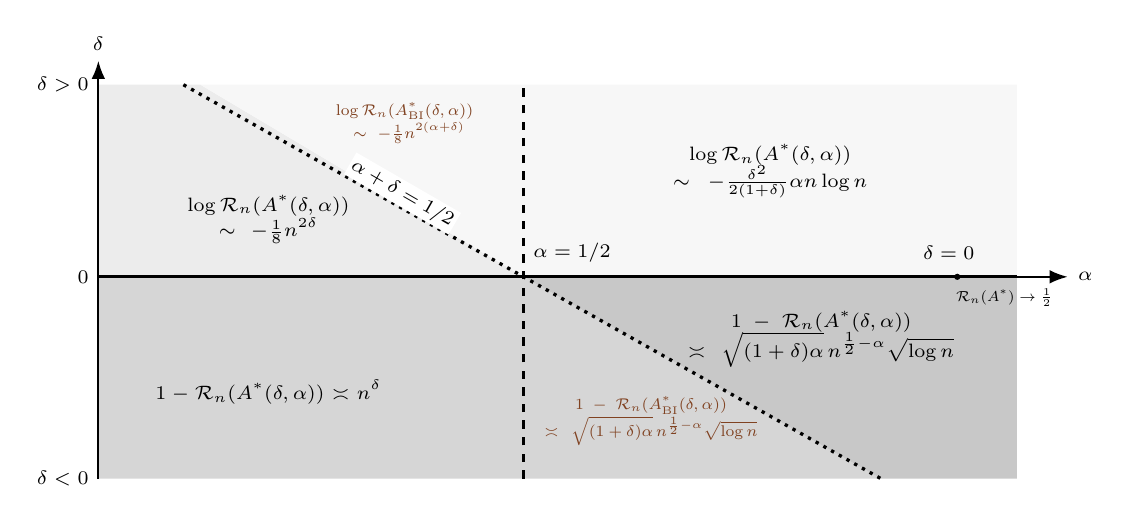
\begin{tikzpicture}[x=10.8cm,y=6.1cm,>=Latex,font=\scriptsize]
    \def\amax{1.08}
    \def\ymax{0.4}
    \def\ymin{-0.42}


    \fill[gray!15]  (0,0) -- (0,\ymax) -- (0.12,\ymax) -- (0.50,0) -- cycle;
    \fill[gray!6] (0.12,\ymax) -- (\amax,\ymax) -- (\amax, 0) -- (0.50,0) -- cycle;
    \fill[gray!32] (0,\ymin) -- (0,0) -- (0.50,0) -- (0.92,\ymin) -- cycle;
    \fill[gray!43] (0.50,0) -- (\amax,0) -- (\amax,\ymin) -- (0.92,\ymin) -- cycle;

    % Axes and phase boundaries.
    \draw[->,thick] (0,\ymin) -- (0,0.45) node[above] {$\delta$};
    \draw[->,thick] (0,0) -- (1.14,0) node[right] {$\alpha$};
    \draw[very thick] (0,0) -- (\amax,0);
    \draw[dashed,thick] (0.50,\ymin) -- (0.50,\ymax);
    \draw[dotted,very thick] (0.1,\ymax) -- (0.50,0) -- (0.92,\ymin);

    % Rate labels. 
    \node[align=center,text width=2.8cm] at (0.2,0.12)
        {$\displaystyle \log\mathcal R_n(A^\ast(\delta, \alpha))$\\[-0.4pt]
         $\displaystyle \sim -\tfrac18 n^{2\delta}$};
     \node[align=center,text width=3.2cm, text = darkbrown, scale = 0.8] at (0.36,0.32)
         {$\displaystyle \log\mathcal R_n(A^\ast_{{\rm BI}}(\delta, \alpha))$\\[0.1pt]
          \hspace{1.5pt} $\displaystyle \sim-\tfrac18 n^{2(\alpha+\delta)}$};
    \node[align=center,text width=4.5cm] at (0.79,0.22)
        {$\displaystyle \log\mathcal R_n(A^\ast(\delta, \alpha))$\\[-1pt]
         $\displaystyle \sim -\tfrac{\delta^2}{2(1+\delta)}\alpha n \log n$};
    \node[align=center,text width=3.1cm] at (0.2,-0.24)
        {$\displaystyle 1-\mathcal R_n(A^\ast(\delta, \alpha)) \asymp n^\delta$};
    \node[align=center,text width=5.1cm] at (0.85,-0.13)
        {$\displaystyle 1-\mathcal R_n(A^\ast(\delta, \alpha))$\\[-1pt]
         $\displaystyle \asymp \sqrt{(1+\delta)\alpha}\,n^{\frac12-\alpha}\sqrt{\log n}$};

    \node[align=center,text width=5.1cm, text = darkbrown, scale=0.8] at (0.65,-0.3)
        {$\displaystyle 1-\mathcal R_n(A^\ast_{{\rm BI}}(\delta, \alpha))$\\[0.1pt]
         $\displaystyle \asymp \sqrt{(1+\delta)\alpha}\,n^{\frac12-\alpha}\sqrt{\log n}$};     

    % Boundary annotations.
    \node[above right] at (0.50,0.01) {$\alpha = 1/2$};
    \node[above,rotate=-30,fill=white,inner sep=1pt] at (0.35,0.15) {$\alpha+\delta=1/2$};
    \node[above] at (1.00,0.015) {$\delta=0$};

    \node[left] at (0,0) {$0$};
    \node[left] at (0,\ymax) {$\delta>0$};
    \node[left] at (0,\ymin) {$\delta<0$};

    % Critical point
    \draw[fill=black] (1.01,0) circle (0.9pt);
    \node[below right, scale=0.75] at (1,-0.01) {$\mathcal R_n(A^\ast)\to \frac12$};
\end{tikzpicture}%
}
\end{center}
\caption{{\bf Phase diagram for the sharp minimax risk.} The horizontal line is the Butucea--Ingster detection boundary. Above it, the displayed rates (in black) describe the decay of $\mathcal R_n(A^\ast(\delta, \alpha))$; below it, they describe the difference $1-\mathcal R_n(A^\ast(\delta, \alpha))$. In each of these half-planes, the asymptotic form of 
$\mathcal R_n(A^\ast(\delta, \alpha))$ changes around the dotted line $\alpha+\delta=1/2$. 
Thus the lines $\delta = 0$ and $\alpha + \delta = 1/2$ split the diagram into four distinct phases for the decay of $\min\{\mathcal R_n(A^\ast(\delta, \alpha)), 1 - \mathcal R_n(A^\ast(\delta, \alpha))\}$ which are color coded in grayscale with darker shade indicating a larger asymptotic order. The rates corresponding to the signal strength $A_{{\rm BI}}^\ast(\delta, \alpha)$ (see \eqref{def:AdeltaBI}) are displayed in {\color{darkbrown}brown} in the two sectors bound between the lines $\alpha + \delta = 1/2$ and $\alpha = 1/2$ which also mark the region such that $A^\ast(\delta, \alpha) \ne A_{{\rm BI}}^\ast(\delta, \alpha)$.}
\label{fig:phase_diagram}
\end{figure}

\smallskip

\noindent\emph{Above the detection boundary.}
When $\delta>0$, the minimax risk tends to zero. In the dense part of the problem, $\alpha + \delta \le1/2$, a global sum test (see \eqref{def:sumscantest} below) is rate-optimal and it is shown in Theorem~\ref{thm:dense_above_boundary} that
\begin{equation}\label{eq:densesupheu}
\log\mathcal R_n(A^\ast(\delta, \alpha))\sim -\frac18 n^{2\delta}.    
\end{equation}
In the sparse sub-regime $\alpha+\delta > 1/2$, the so-called scan statistic (cf.~\eqref{def:sumscantest}) yields the optimal rate and we obtain in part~1 of Theorem~\ref{thm:sparse_riskbnd} that
\begin{equation}\label{eq:sparsesupheu}
\log\mathcal R_n(A^\ast(\delta, \alpha)) \sim -\frac{\delta^2}{4(1+\delta)} \log |\mathcal S|,
\end{equation}
where $\mathcal S$ is the set of all $n\times n$ submatrices of $[N]\times[N]$. Since $\log|\mathcal S|=(1+o(1))2\alpha n\log n$, this gives the minimax risk to the principal exponential order.

\vspace{0.1cm}

In an alternative interpretation of the detection boundary adopted by 
\cite{butuceasubmatrix2013} (see above Remark~2.1 in the paper), one can first determine the boundary threshold $A^\ast(0, \alpha)$ which changes its form according to \eqref{def:Adelta} around the critical value $\alpha_c = 1/2$ and then vary it with 
respect to the parameter $\delta$ in the manner consistent with this form (see 
below). More precisely, with
\begin{equation}\label{def:AdeltaBI}
A^\ast_{{\rm BI}}(\delta, \alpha) = A^\ast_{{\rm BI}}(\delta, \alpha; n) \stackrel{{\rm def.}}{=} 
    \begin{cases}
        n^{-(1 - \alpha - \delta)}, & \alpha \le 1/2,\\
        \sqrt{\frac{4(1+\delta)\alpha\log n}{n}}, & \alpha > 1/2,
    \end{cases} \qquad \mbox{for } \delta\in(-1,\infty),
\end{equation}
the results of \cite{butuceasubmatrix2013} yield that $\mathcal R_n(A^\ast_{{\rm BI}}(\delta, \alpha)) \to 0/1$ for $\delta \gtrless 0$ respectively. It is a natural question to ask how the 
phase diagrams for these two signal strength profiles are related. Note that we can have 
$A^\ast_{{\rm BI}}(\delta, \alpha) \neq A^\ast(\delta, \alpha)$ for some $\delta > 0$ {\em only if} $\alpha + \delta > 1/2 \ge \alpha$. In Figure~\ref{fig:phase_diagram}, this corresponds to the sector above the diagonal line $\alpha + \delta = 1/2$ in the second quadrant. It turns out 
that a scan test is still rate-optimal in this sub-regime and we establish in part~2 of 
Theorem~\ref{thm:sparse_riskbnd}:
\begin{equation}\label{eq:densesupBIheu}
\log\mathcal R_n(A^\ast_{{\rm BI}}(\delta, \alpha))\sim -\frac18 n^{2(\alpha+\delta)}.
\end{equation}
 

\smallskip

\noindent\emph{Below the detection boundary.}
When $\delta < 0$, the minimax risk 
tends to 1. Theorems~\ref{thm:dense_below_boundary} and \ref{thm:sparse_below_boundary} show 
that the deficit from 1 is {\em polynomial} rather than (stretched or 
super-)exponentially small. In the dense below-boundary (sub-)regime $\alpha+\delta\le1/2$, 
a sum test statistic achieves the optimal rate like in the dense above-boundary regime 
discussed above (but for a new threshold) and we show in 
Theorem~\ref{thm:dense_below_boundary} that
\begin{equation}\label{eq:densesubheu}
1-\mathcal R_n(A^\ast(\delta, \alpha))\asymp n^{\delta},
\end{equation}
with absolute implicit constants. This would suggest that the optimal rate in the sparse 
below-boundary regime $\alpha + \delta > 1/2$ should come from a scan test as 
in the \sloppy sparse above-boundary regime. Surprisingly, this heuristic turns out to be {\em false} and the same sum test still attains the optimal rate which we 
identify in Theorem~\ref{thm:sparse_below_boundary} as
\begin{equation}\label{eq:sparsesubheu}
1-\mathcal R_n(A^\ast(\delta, \alpha))
    \asymp \sqrt{(1+\delta)\alpha}\, n^{1/2-\alpha}\sqrt{\log n},
\end{equation}
again up to absolute multiplicative constants. In fact, the same rate continues to 
hold for {\em any} $\alpha > 1/2$ and thus \eqref{eq:sparsesubheu} remains valid 
upon replacing $A^\ast(\delta, \alpha)$ with $A^\ast_{{\rm BI}}(\delta, \alpha)$ when $\alpha > 1/2 \ge \alpha + \delta$ which is precisely the region where $A^\ast(\delta, \alpha) \neq A^\ast_{{\rm BI}}(\delta, \alpha)$ for $\delta < 0$ (revisit \eqref{def:AdeltaBI} above and see Figure~\ref{fig:phase_diagram}).



\smallskip

\noindent\emph{On the boundary.}
Finally, Theorem~\ref{thm:criticality} treats a fixed-$n$ very sparse critical regime in which $A^\ast = \sqrt{4\log N/n}$ (note that $\alpha \log n = \log \frac Nn$ for $N = n^{1 + \alpha}$ in \eqref{def:Adelta}). In this case, 
Theorem~\ref{thm:criticality} tells us that
\begin{equation}\label{eq:sparsecritheu}    
\lim_{n \to \infty} \mathcal R_n(A^\ast) = \frac12.
\end{equation}
Thus the critical behavior is genuinely non-degenerate in this scaling. This 
behavior is also markedly {\em different} from the sparse Gaussian 
sequence model and the linear regression model \citep{ingster2012nonparametric, mukherjee2020minimax} where the minimax risk for detecting $s$-sparse signals at 
criticality converges to $\frac1{2^s}$ for fixed $s$. Therefore, whereas the 
minimax risk at criticality for sparse vector signal detection decreases with the 
size of the (sparse) signal, the minimax risk at criticality for detecting fixed-sized sub-matrices does not depend on the submatrix size. We will see in 
\eqref{eq:sparsecritheud} below that the same limiting value $\frac12$ holds for 
the tensor version for the problem as well.

\smallskip

\noindent\emph{Extension to subtensor detection.} One can similarly consider 
the problem of detecting an $n \times \ldots \times n$ dimensional order-$d$ tensor embedded in a larger $N \times \ldots \times N$ tensor for any $d \ge 2$ ($d = 2$ being the matrix case). The corresponding detection boundary was identified in \cite{MR4382029} as stated below:
 \begin{equation}\label{def:Adelta_tensor}
A^\ast_d(\delta, \alpha) = A^\ast_d(\delta, \alpha; n)\stackrel{{\rm def.}}{=}
\min\left\{n^{-\frac d2(1-\alpha-\delta)},
\sqrt{\frac{2d(1+\delta)\alpha\log n}{n^{d-1}}}\right\},
\qquad \delta\in(-1,\infty).
\tag{\ref{def:Adelta}$'$}
\end{equation}
In this case the critical line demarcating the dense/sparse transition becomes 
$\alpha + \delta = 1/d$. Our proofs along with the dichotomy between sum/scan 
mechanism for $d = 2$ carry over, {\em mutatis mutandis}, to any general $d$. 
Therefore, to keep our exposition uncluttered, we only state (and prove) our main results in 
the upcoming section(s) for matrices while recording the results for the general 
order-$d$ case below


In the dense above-boundary regime, namely $\alpha + \delta \le 1/d$ and $\delta > 
0$, the minimax risk behaves like 
\begin{equation}\label{eq:densesupheud}
\log\mathcal R_n(A^\ast_d(\delta, \alpha)) \sim -\frac18 n^{d\delta}
\tag{\ref{eq:densesupheu}$'$}
\end{equation}
where, by slightly abusing the notation, we continue to use $\mathcal R_n( \cdot )$ for the minimax risk of the general testing problem. On the other hand, in the sparse above-boundary 
regime given by $\alpha + \delta > 1/d$ and $\delta > 0$, we have
\begin{equation}\label{eq:sparsesupheud}
\log\mathcal R_n(A^\ast_d(\delta, \alpha)) \sim -\frac{\delta^2}{4(1+\delta)} \log |\mathcal S_d|,    
\tag{\ref{eq:sparsesupheu}$'$}
\end{equation}
where $\mathcal S_d$ denotes the set of all $n\times \ldots \times n$ order-$d$ 
subtensors of $[N] \times \ldots \times [N]$. This is identical to the matrix, i.e., $d = 2$ case except that now we have $\log|\mathcal S_d|=(1+o(1))d\alpha n\log n$. 

We can also define a signal strength function $A^\ast_{d, {\rm BI}}(\delta, \alpha)$ 
analogous to \eqref{def:AdeltaBI}. Similar to the matrix version (with $d$ in place of 2), we have $A^\ast_{d, {\rm BI}}(\delta, \alpha) \ne A^\ast_{d}(\delta, \alpha)$ for some $\delta > 0$ only if $\alpha + \delta > 1/d \ge \alpha$, in which case 
\begin{equation}\label{eq:densesupBIheud}
\log\mathcal R_n(A^\ast_d(\delta, \alpha))\sim -\frac18 n^{d(\alpha+\delta)}.
\tag{\ref{eq:densesupBIheu}$'$}
\end{equation}

\vspace{0.15cm}

Below the detection boundary, the risks again exhibit power-law decay around the limiting 
value 1. In the dense below-boundary regime $\alpha + \delta \le 1/d$, we get
\begin{equation}\label{eq:densesubheud}
1-\mathcal R_n(A^\ast_d(\delta, \alpha))\asymp n^{d\delta/2}
\tag{\ref{eq:densesubheu}$'$}
\end{equation}
while for all $\alpha > 1/d$, we have
\begin{equation}\label{eq:sparsesubheud}
1-\mathcal R_n(A^\ast_d(\delta, \alpha))
    \asymp \sqrt{(1+\delta)\alpha}\, n^{1/2 - d\alpha/2}\sqrt{\log n}.
\tag{\ref{eq:sparsesubheu}$'$}    
\end{equation}
The multiplicative constants implicit in ``$\asymp$'' involve $d$ for both the 
bounds.

\vspace{0.1cm}

Finally, in the fixed-$n$ sparse critical regime, the detection threshold is 
$A^\ast_d = \sqrt{2d\log N/n}$ and 
\begin{equation}\label{eq:sparsecritheud}    
\lim_{n \to \infty} \mathcal R_n(A^\ast_d) = \frac12.
\tag{\ref{eq:sparsecritheu}$'$} 
\end{equation}
Thus the critical limiting minimax risk in the fixed-size setting neither depends on $n$ {\em nor} on the order $d$ of the tensor.


\subsection{Proof overview}\label{subsec:overview}
Let
\begin{equation}\label{def:Sfamily}
\mathcal S = \mathcal S(n; \alpha) \stackrel{{\rm def.}}{=}
\{\cR\times\cC\subset[N]\times[N]: |\cR|=|\cC|=n\}
\end{equation}
and for $S\in\mathcal S$ or, more generally, $S \subset [N] \times [N]$, write
\begin{equation}\label{def:XS}
X_S\stackrel{{\rm def.}}{=}\sum_{(i,j)\in S}X_{ij}.    
\end{equation}
The upper bounds on the minimax risks arise from two different types of test statistics, namely 
\begin{equation}\label{def:sumscantest}
T_{{\rm sum}}^H  \stackrel{{\rm def.}}{=} \mathbf{1}_{\{X_{[N]\times[N]} > H\}} \,\, \mbox{ and } \,\, T_{{\rm scan}}^H \stackrel{{\rm def.}}{=} \mathbf{1}_{\big\{\max\limits_{S\in \mathcal{S}} \frac{X_{S}}n > H \big\}}
\end{equation}
referred to as the {\em sum} test and the {\em scan} test respectively w.r.t. the threshold $H$ (with implicit dependence on $n$). The same statistics were also used 
for constructing ``good'' tests in \cite{butuceasubmatrix2013}. For any choice of 
the signal strength $A$, computing the optimal value of $H = H_n(A)$ that minimizes the maximum risk for either of 
these tests is rather straightforward and usually involves, as in the case of $T_{{\rm scan}}$, a standard first-moment 
computation. Thus we can generate ``reasonable'' upper bounds on the minimax risk in this manner with an important caveat that the choice between the two types of tests 
may be different in the below-boundary regime (where all tests are ``bad'', see below) from its above-boundary counterpart. The main and the much more difficult 
part is to show that these rates are optimal over all possible tests.

\vspace{0.15cm}

A classical lower bound on the minimax risk is given by the minimum {\em Bayes risk} under some suitable prior $p$ on the parameter space $\Theta(A) = \Theta(A, n)$ (recall \eqref{def:Theta}). By the Neyman-Pearson lemma, the minimum Bayes 
risk is attained by the corresponding likelihood ratio test, i.e., the statistic $\mathbf{1}_{\{L_{p} > 1\}}$ where $L_{p}$ denotes the integrated likelihood ratio under $p$. In view of the obvious ``monotonicity'' of the probability 
measures indexed by $\Theta(A)$ with respect to $(\theta_{ij})_{1 \le i, j \le N}$, 
we can choose, as $p$, the uniform prior $\bpi$ on the boundary of $\Theta(A)$, i.e., the set
\begin{equation}\label{def:partialTheta}
    \partial \Theta(A) \stackrel{{\rm def.}}{=} \big\{\btheta:\exists\ \cR\subset[N],\ \cC\subset[N],\ |\cR| = n,\ |\cC| = n,
\theta_{ij} = A\mathbf 1_{(i,j)\in \cR\times\cC}\big\}
\end{equation}
(cf.~\eqref{def:Theta}). The corresponding integrated likelihood ratio (recall \eqref{def:Xdist}; see also \eqref{eq:Lpiform}) is
\begin{equation}\label{def:Lpi}
L_{\bpi}=\frac1{|\mathcal S|}\sum_{S\in\mathcal S}
\exp\left(A X_S-\frac{A^2 n^2}{2}\right).
\end{equation}
The core lower-bound problem is to estimate the lower tail of this likelihood 
ratio under $\P_0$.

One obvious problem that one faces in analyzing \eqref{def:Lpi} is that the summands 
comprising $L_{\bpi}$ are far from being independent. Indeed, the second moment of 
$L_{\bpi}$ is governed by overlaps and can be expressed as
\begin{equation*}
\E_0(L_{\bpi}^2)  = \frac1{|\mathcal S|} \sum_{1 \le k, \ell \le n} \exp(A^2k\ell) N_{k, \ell}
\end{equation*}
where $N_{k, \ell}$ denotes the number of submatrices intersecting a given submatrix 
with number of common rows and columns $k$ and $\ell$ respectively. In most 
situations of interest, this second moment blows up. To remedy this, 
\cite{butuceasubmatrix2013} introduces a ``blanket'' truncation of $L_{\bpi}$; see 
\eqref{def:LpiE} below for a generic form of such truncations. The truncated second 
moment typically looks like
\begin{equation}\label{eq:trunc_secmom}
\frac1{|\mathcal S|} \sum_{1 \le k, \ell \le n} \exp( q(k\ell, A) ) \, N_{k, \ell}
\end{equation}
where the function $q(k\ell, A) = q(k\ell, A; n)$ depends on the underlying 
truncation. The truncation in \cite{butuceasubmatrix2013} allows the authors to show 
that the limiting minimax risk is 1 in the below-boundary regime. However, we cannot
hope to capture the sharp rates and their complex phase transition as revealed by 
Figure~\ref{fig:phase_diagram} with a {\em single} choice of truncation. Before 
elaborating on this further, let us note that \eqref{eq:trunc_secmom} can be 
interpreted as a {\em partition function} for a Gibbs measure on the overlap 
patterns $(k, \ell)$ with $q(k\ell, A)$ contributing the energy terms. 
This interpretation is not merely speculative. Indeed, in the above-boundary regime, 
our sharp exponential rates correspond to the {\em free energy} for such energy-entropy pairing. We now comment very briefly on the proofs for each of the four 
phases in Figure~\ref{fig:phase_diagram}. 


\vspace{0.15cm}

\noindent{{\em Dense above-boundary regime}.} In this regime, the upper bound follows 
from a sum test. For the lower bound, we apply a Cauchy--Schwarz/Paley--Zygmund type 
argument to $L_{\bpi}$ restricted to a typical event for the sum statistic. As hinted above, the exponent $n^{2\delta}/8$ is produced by a free energy computation 
where the entropy-energy functional $q(k\ell, A) + \log N_{k, \ell}$ (cf.~\eqref{eq:trunc_secmom}) is maximized at essentially typical overlaps of order 
$n^2/N$.

\vspace{0.1cm}

\noindent{{\em Sparse above-boundary regime}.} In this case, the optimal upper bound is obtained by a scan statistic. For the lower bound, we first compare the 
likelihood ratio to the maximum of $X_S$ over $S\in\mathcal S$. The problem is then 
reduced to a second-moment estimate for the number of exceedances of a ``high level'' by $X_S; S \in \mathcal S$. A careful free energy-type computation then 
shows that the dominant contribution has exponent $\frac{\delta^2}{4(1+\delta)}$ on 
the scale $\log|\mathcal S|$.

\vspace{0.1cm}

\noindent{{\em Dense and sparse below-boundary regime}.} Below the boundary, the object of interest is the small difference $1-\mathcal R_n(A)$. Interestingly, the upper bounds in both dense and sparse regimes 
come from the same sum test while the lower bounds use 
Lemma~\ref{lem:risk_lowerbnd_ab}, a general lower bound in terms of first and second 
moments of truncated-likelihood with very different choices of truncation. A crucial 
difference from the above-boundary phase is that the ``free energy principle'' no 
longer holds and the variance of the truncated-likelihood decays at a much slower 
power-law rate contributed by several terms rather than a single dominant term. This 
is visible in the polynomial rates for $1 - \mathcal R_n(A)$. The proof for the 
sparse case is particularly delicate.

\vspace{0.1cm}

\noindent{{\em Critical fixed-size regime}.} The result in the critical regime uses 
a truncated likelihood ratio similar to the sparse below-boundary regime and shows that, for fixed $n$, all non-identical overlap pairs become negligible while the 
truncation removes exactly half of the planted mass, yielding the limit $1/2$.

\subsection{Organization} Section~\ref{sec:main_results} states the main theorems.  Section~\ref{sec:discussions} discusses related problems, adaptation, computational considerations, and future directions. Section~\ref{sec:prelim} collects combinatorial estimates, normal tail bounds, and the truncated-likelihood lower bound. Sections~\ref{sec:dense_above}--\ref{sec:criticality} contain the proofs of the main results.

\subsection{Notation} We write $c,c',C,C'$ for finite positive constants whose 
values may change from line to line. Unless indicated otherwise, constants are 
absolute; dependence on parameters such as $\alpha > 0$ and $\delta \in \R$ (see \eqref{eq:mnregime} and \eqref{def:Adelta}) is displayed when relevant. We will also suppress the dependence of a specific test $T_n$ as well as the parameter space $\Theta(A, n)$ (cf.~\eqref{def:Theta}) on the underlying scale parameter 
$n$, as the latter would be clear from the context. We use the notation $[M]$ for 
the set of integers $\{1,\ldots, M\}$ for any positive integer $M$. The limits as 
$n \to \infty$ are always taken with $\alpha$ and $\delta$ fixed. In the same 
vein, we use $o(1)$ to denote any function of $n$ (depending possibly on $\alpha$ 
and $\delta$) that tends to $0$ as $n \to \infty$ with $\alpha$ and $\delta$ 
fixed. We denote the joint distribution of $\bX$ under the mean matrix $\btheta \in \R^{N \times N}$ as $\P_{\btheta}$ and the corresponding expectation, variance 
as $\E_{\btheta}, \mathrm{Var}_{\btheta}$ respectively (see \eqref{def:Theta}--\eqref{eqn:bayes_risk}). When $\btheta = \mathbf 0$, i.e., the mean matrix 
corresponding to the null distribution, we use the (slightly) simplified notations 
$\P_0, \E_0$ and ${\rm Var}_0$.
 

\section{Main Results} \label{sec:main_results}
We now state the precise risk asymptotics. Recall the notation \sloppy $\mathcal R_n(A)=\inf_T\mathrm{Risk}(T,A,n)$ and the family $\mathcal S$ of $n\times n$ 
submatrices of $[N]\times[N]$ from \eqref{def:Sfamily}.

\subsection{Above-boundary regime $(\delta>0)$}\label{subsec:main_above_bnd}
The first theorem concerns the dense side of the phase diagram where $\alpha + \delta \le 1/2$. In this part, the signal 
strength $A^\ast(\delta, \alpha)$ as given by \eqref{def:Adelta} is the algebraic rate $n^{-(1-\alpha-\delta)}$. %and the optimal test is a sum test (see \eqref{def:sumscantest}).
\begin{theorem}[Dense above-boundary regime]\label{thm:dense_above_boundary}
Let $\alpha + \delta \leq 1/2$ and $\delta>0$. %and let$A(\delta)=n^{-(1-\alpha-\delta)}$.
Then
\begin{equation}\label{eq:dense_riskbnd1}
\lim_{n\to\infty}
\frac{\log \mathcal R_n(A^\ast(\delta, \alpha))}{n^{2\delta}}
=-\frac18.
\end{equation}
\end{theorem}



The next theorem covers the sparse scan-dominated sub-regime. We state it for $\alpha + \delta > 1/2$, where this is the Butucea--Ingster sparse regime, but the proof gives the same exponent for {\em every} fixed $\alpha > 0$ if the sparse regime signal strength $A^\ast(\delta, \alpha) = \sqrt{4(1+\delta)\alpha\log n / n}$ (recall \eqref{def:Adelta}) is used. We also give the asymptotic rate corresponding to the signal strength $A^\ast_{{\rm BI}}(\delta, \alpha) = n^{-(1 - \alpha -\delta)}$ for 
$\alpha + \delta > 1/2 \ge \alpha$ which defines the region where $A^\ast_{{\rm BI}}(\delta, \alpha)$ and $A^\ast(\delta, \alpha)$ are not equal for $\delta > 0$ (see \eqref{def:AdeltaBI} and the surrounding discussion in \S\ref{subsec:summary}). 
\begin{theorem}[Sparse above-boundary regime]\label{thm:sparse_riskbnd}
Let $\alpha + \delta > 1/2$ and $\delta > 0$.
\begin{enumerate}
\item We have
\begin{equation}\label{eq:sparse_riskbnd}
\lim_{n\to\infty}
\frac{\log\mathcal R_n(A^\ast(\delta, \alpha))}{\log|\mathcal S|}
=-\frac{\delta^2}{4(1+\delta)}
\end{equation}
and the same conclusion holds for all $\alpha > 0$ and the same choice of signal 
strength.
\item If also $\alpha \le 1/2$, then
\begin{equation}\label{eq:dense_riskbnd2}
\lim_{n\to\infty}
\frac{\log \mathcal R_n(A^\ast_{{\rm BI}}(\delta, \alpha))}{n^{2(\alpha+\delta)}}
=-\frac18.
\end{equation}
\end{enumerate}
\end{theorem}
% \begin{thmbis}{thm:dense_above_boundary}
% aas
% \end{thmbis}

Since $\log|\mathcal S|=(1+o(1)) \, 2\alpha n\log n$ (see \eqref{eq:Scardinality} below), part~1 of Theorem~\ref{thm:sparse_riskbnd} determines the minimax risk up 
to the principal exponential order. The proof of part~2 is essentially a 
corollary of the proof of part~1.


\subsection{Below-boundary regime $(\delta < 0)$}\label{subsec:main_below_bnd}
Below the detection boundary, the minimax risk tends to 1. The following two theorems quantify the size of the quantity $1-\mathcal R_n(A^\ast(\delta, \alpha))$. The first result below characterizes the case when $\alpha+\delta\leq\frac{1}{2}$ -- which can arise when $\alpha\leq \frac{1}{2}$ or $\alpha>\frac{1}{2}$ but $\delta$ negative enough. 
\begin{theorem}[Dense below-boundary regime]\label{thm:dense_below_boundary}
Let $\alpha+\delta\le1/2$ and $\delta < 0$. Then
\begin{equation}\label{eq:dense_below_boundary0}
\lim_{n\to\infty}
\frac{\log(1-\mathcal R_n(A^\ast(\delta, \alpha)))}{\log n} =\delta.
\end{equation}
More precisely, there exist absolute constants $c,C\in(0,\infty)$ and $n_0(\alpha,\delta)<\infty$ such that, for all $n\ge n_0(\alpha,\delta)$,
\begin{equation}\label{eq:dense_below_boundary}
    c\le
    \frac{1-\mathcal R_n(A^\ast(\delta, \alpha))}{n^\delta}
    \le C.
\end{equation}
\end{theorem}
Next, we move on to the sparse sub-regime, i.e., $\alpha + \delta > 1/2$ which implies 
that $\alpha > 1/2$ since $\delta < 0$. Somewhat like the part~1 of Theorem~\ref{thm:sparse_riskbnd}, the rate given by Theorem~\ref{thm:dense_below_boundary} below holds for all $\alpha > 1/2$ provided 
the sparse regime signal strength $A^\ast(\delta, \alpha) = 
\sqrt{4(1+\delta)\alpha\log n / n}$ is used. Now note from \eqref{def:AdeltaBI} that $A^\ast_{{\rm BI}}(\delta, \alpha) = \sqrt{4(1+\delta)\alpha\log n / n}$ when $\alpha > 1/2 \ge \alpha + \delta$. But this is also the region where $A^\ast_{{\rm BI}}(\delta, \alpha)$ and $A^\ast(\delta, \alpha)$ are different for $\delta < 0$. 
Thus Theorem~\ref{thm:dense_below_boundary} covers the analog of Theorem~\ref{thm:sparse_riskbnd}, part~2 in this regime.
\begin{theorem}[Sparse below-boundary regime]\label{thm:sparse_below_boundary}
Suppose that $\alpha>1/2$, $\delta\in(-1,0)$ and $A(\delta, \alpha) = \sqrt{4(1+\delta)\alpha\log n / n}$. Then
\begin{equation}\label{eq:sparse_below_boundary0}
\lim_{n\to\infty}
\frac{\log(1-\mathcal R_n(A(\delta, \alpha)))}{\log n}
=\frac12-\alpha.
\end{equation}
Moreover, there exist absolute constants $c,C\in(0,\infty)$ and $n_0(\alpha,\delta)<\infty$ such that, for all $n\ge n_0(\alpha,\delta)$,
\begin{equation}\label{eq:sparse_below_boundary}
    c\le
    \frac{1-\mathcal R_n(A(\delta, \alpha))}{\sqrt{(1+\delta)\alpha}\,n^{1/2-\alpha}\sqrt{\log n}}
    \le C.
\end{equation}
\end{theorem}

Theorems~\ref{thm:dense_below_boundary} and \ref{thm:sparse_below_boundary} reveal a qualitatively different behavior compared to the above-boundary phase studied in 
Theorems~\ref{thm:dense_above_boundary} and \ref{thm:sparse_riskbnd}. Specifically, the minimax risks approach their limiting value at a much slower polynomial rate, rather than at a stretched or super-exponential speed. This distinction is also reflected in the proof mechanisms for the two regimes, particularly in the lower bounds. While the above-boundary rates emerge from a single free energy-like term dominating the second moment of a suitably truncated statistic (e.g., the likelihood ratio), the below-boundary rates result from the combined contributions of several distinct terms; see \S\ref{subsec:overview} for more details. 


\subsection{Critical regime $(\delta=0)$}\label{subsec:main_on_bnd}
We finally record a critical result in a fixed-submatrix-size sparse regime. Here 
$n$ remains bounded and $N$ grows to $\infty$ although our proof can be easily 
adapted to accommodate the regime where $n$ grows sufficiently slowly as a 
function of $N$. Since we are working in the extremely sparse limit (i.e., $\alpha = \infty$), the value of the threshold $A^\ast$ corresponding to \eqref{def:Adelta} in 
this case is given by $\sqrt{\tfrac{4\log N}{n}}$ (note that $\alpha \log n = \log 
\frac Nn$ when $N = n^{1 + \alpha}$).
\begin{theorem}[A fixed-size critical limit]\label{thm:criticality}
For any fixed $n$ and $A^\ast = \sqrt{4\log N/n}$,
\begin{equation}\label{eq:lim_critical}
\lim_{N\to\infty} \mathcal R_n(A^\ast) = \frac12.
\end{equation}
\end{theorem}
Results of similar flavor have appeared previously in the context of Gaussian 
sequence models \citep[Theorem~8.1]{ingster2012nonparametric} and linear 
regression models \citep[Theorem~2.5]{mukherjee2020minimax}. However, 
\eqref{eq:lim_critical} is different from these results as the limiting value does 
{\em not} depend on the size of the signal $n$.



\section{Discussions and Open Directions}\label{sec:discussions}
\subsection{Connections to existing literature} The results in this paper are 
connected to both the classical foundations of statistical efficiency theory and 
recent research on sparse signal detection. We expand on them below. We refer the 
reader to \cite[Section~1.4]{mukherjee2020minimax} for more detailed discussions 
in a related context.

\subsubsection{Connections to Chernoff exponents and Bahadur efficiency} The viewpoint adopted here is also related to the classical theory of asymptotic error exponents in hypothesis testing.  For testing a fixed simple null $P$ against a fixed simple alternative $Q$ from $m$ independent observations, the optimal sum of the two errors is governed, on the exponential scale, by the Chernoff-exponent
\begin{equation*}
   -\inf_{0\le \lambda \le1} \log \int \left(\frac{dQ}{dP}\right)^{\lambda} dP,
\end{equation*}
see, e.g., \cite[Corollary~12.1]{polyanskiy2014lecture}. Bahadur's efficiency 
gives another large-deviation comparison of tests, in which the relevant quantity 
is the exponential rate at which attained significance levels decay under 
alternatives; see, for instance, \cite{bahadur1967rates}. Both theories ask for 
more than consistency: they compare tests by the speed at which their error 
probabilities, or related tail probabilities, become small. In this regard, our results can be 
viewed as providing an analog of Chernoff exponent and Bahadur efficiency for sparse 
submatrix detection problems.

There are two important differences in the present setting.  First, the sparse submatrix problem is composite rather than simple-versus-simple.  The likelihood ratio that enters the lower bounds is therefore an integrated likelihood ratio over a least favorable prior on submatrices, not a product of i.i.d. one-observation likelihood ratios. Second, the null and alternative approach one another with $n$ and $N$, and hence the error need not decay exponentially on the sample-size scale.  Indeed, the present results show three distinct behaviors: stretched- or super-exponential decay of $\mathcal R_n(A^\ast(\delta, \alpha))$ above the boundary, polynomial decay of $1-\mathcal R_n(A^\ast(\delta, \alpha))$ below the boundary, and a non-degenerate limiting risk at criticality.

\subsubsection{Connections to Bhattacharyya affinity} Another useful way to view the minimax risk is through the affinity between the null distribution and a suitably averaged alternative. If $\P_p = \int \P_{\btheta}\,d p(\btheta)$ is the mixture induced by a prior $p$ on 
planted submatrices, the Bhattacharyya affinity is
\begin{equation*}
\rho(\P_0, \P_p) = \E_0\sqrt{L_p},
\end{equation*}
where $L_p = d\P_{p}/d\P_0$. This quantity directly controls the Bayes testing risk and is 
often more closely tied to the optimal testing error than the second moments of likelihood 
ratios; see, e.g., \cite{bhattacharyya1946measure,addarioberry2010combinatorial}. In particular, controlling the affinity  could give a conceptually clean route to sharp lower bounds.

For sparse submatrix detection, however, the affinity is difficult to evaluate directly. The integrated likelihood ratio is a highly dependent average over $\binom{N}{n}^2$ possible submatrices, and its tails are governed by rare but influential pairs of submatrices with atypically large overlaps. In a sense, the technical core of the paper may be regarded as a way to understand the Bhattacharyya affinity, carried out through more tractable second-moment analysis.

\subsubsection{Connections to sparse Gaussian mixture models} The sparse Gaussian mixture model is a closely related benchmark for rare/weak signal detection.  In its simplest form one observes independent variables from
\begin{equation*}
    H_0:\;Y_i\sim N(0,1),
    \qquad
    H_1:\;Y_i\sim (1-\varepsilon_n)N(0,1)+\varepsilon_n N(\mu_n,1),
\end{equation*}
and asks for the detection boundary or for sharper error asymptotics.  The detection-boundary theory for such models is classical in the higher-criticism literature \cite{donoho2004higher,cai2011optimal,caiwu2014optimal,ariascastro2019sparse}.  More recently, \cite{ligo2016detecting} studied the rate of decay of error probabilities for sparse mixtures in {\em some} regimes, showing that the relevant decay can be sublinear in the number of observations and can be governed by divergence quantities different from those in the non-sparse case. 

However, for the question of interest in this paper, the problems of sparse Gaussian mixtures and sparse submatrix detection are very different.  In the mixture model, the likelihood ratio factorizes over observations, so one can often reduce the analysis to large deviations for sums of independent random variables. In the submatrix model, the unknown signal is a combinatorial object with row and column structure; two alternatives are not independent labels but overlapping submatrices. The resulting entropy--energy balance over overlap sizes is responsible for the secondary transition at $\alpha + \delta = 1/2$ and for the distinction between sum- and scan-dominated regimes.

\subsection{Comparisons with \cite{mukherjee2020minimax}}
A particularly close conceptual antecedent to the present work is the paper of
\cite{mukherjee2020minimax} on minimax exponents for sparse testing in
high-dimensional linear regression.  That paper asks the same broad
second-order question which motivates the present article: once the usual
detection boundary is known, what is the sharp asymptotic size of the minimax
testing risk itself?  Thus the two papers belong to the same general program of refining
detection-boundary theory into a theory of sharp risk asymptotics.

The similarity, however, is at the level of this general program rather than at
the level of the mathematical model.  The work of \cite{mukherjee2020minimax}
concerns sparse alternatives in high-dimensional linear regression; in the
orthogonal-design case, this reduces essentially to a Gaussian sequence model,
while for random designs the size and distribution of the design matrix enters the analysis.
The present paper concerns the square sparse-submatrix model of 
\cite{butuceasubmatrix2013} where the (relevant) alternatives are parametrized by submatrices rather than ``unstructured'' subsets of $[N] \times [N]$. The underlying product structure is crucial for the entropy--energy balance driving the secondary 
transition at $\alpha+\delta=1/2$. The distinctive role played by such a structure becomes 
even clearer from the tensor extension recorded in \S\ref{subsec:summary}.  The same 
methods extend to detecting an $n\times\cdots\times n$ order-$d$ elevated subtensor 
inside an $N\times\cdots\times N$ Gaussian tensor, for every fixed $d\ge2$.  In that
setting the detection boundary changes in the natural way, the secondary
dense/sparse transition line becomes $\alpha+\delta=1/d$, and the {\em complete}
above-boundary, below-boundary, and fixed-size critical risk picture persists. %These behaviors are very different from their counterparts, {\em conjecturally} in several regimes for the risks (see below and also Figures~1 and ), in the high-dimensional regression problem.
Thus the matrix case should be viewed as the 
first member of the order-$d$ sub-tensor detection problem with $d \ge 2$, as opposed to 
an extension of the Gaussian sequence-type models. 


The scope and sharpness of the results are also different. \cite{mukherjee2020minimax} 
obtain a set of sharp exponent results, but their Section~4 explicitly identifies two
parameter regions in which the minimax risk remains uncharacterized. By
contrast, for the canonical square submatrix model, and more generally for the
corresponding fixed-order tensor extensions described above, the present work
gives a {\em closed} phase diagram across the above-boundary, below-boundary, and
critical regimes. %Also our estimates in the below-boundary regime are correct up to absolute multiplicative constants, whereas \cite{mukherjee2020minimax} establish logarithmic orders for the corresponding terms.
%The comparison should therefore not be read as a comparison
%of difficulty between the two models.  Rather, the two papers exhibit different
%manifestations of a common phenomenon: first-order detectability can conceal a
%much richer structure in the actual minimax risk.  The contribution of the
%present article is to carry out this program for product-structured sparse
%submatrix and subtensor detection, where overlap geometry leads to a complete
%multi-level phase diagram.

\subsubsection{Computational considerations}
The minimax results here are information-theoretic.  In the scan-dominated regimes, the natural optimal procedure involves maximizing $X_S$ over all $S\in\mathcal S$, which is computationally infeasible in the worst case.  Computational-statistical tradeoffs for submatrix detection were studied by \cite{ma2015computational}, who related efficient detection to planted-clique-type barriers in certain regimes (see also the more recent work \cite{MR4928482}).  More broadly, similar computational gaps are known or conjectured in sparse PCA and related planted-structure problems; see, for example, \cite{berthet2013complexity}.

The sharp-risk point of view raises a more refined computational question. Do the polynomial-time tests achieve the same large-deviation exponent above the boundary or the same polynomial difference (from $1$) below it? Conversely, can one prove computational lower bounds at the level of risk exponents rather than merely at the level of zero-one detectability? 

\subsection{Other models and further directions}\label{subsec:directions}
Several extensions are natural. First, one could study rectangular submatrices with $n\ne m$ and ambient dimensions $N\ne M$ with possibly different values of the exponent $\alpha$ in each dimension, where additional regimes may appear.  Second, it would be interesting to develop a full critical-window theory, allowing $n\to\infty$ and perturbing $A$ at scales finer than those considered here.  Third, analogous sharp-risk questions can be asked for non-Gaussian exponential-family noise, unknown variance, two-sided alternatives, and heterogeneous signal amplitudes.  Finally, the free energy structure of the truncated second moment suggests possible connections with sharper large-deviation principles for overlap distributions in other high-dimensional testing problems.

\section{Preliminaries}\label{sec:prelim}
In this section we gather some results that are used repeatedly throughout our 
proofs. Lemma~\ref{lem:factorial} and the subsequent Corollary~\ref{cor:factorial} 
provide ``manageable'' expressions for certain counts of submatrices %of $[N] \times [N]$ 
which are crucial for obtaining minimax lower bounds via second moment 
computations. In Lemma~\ref{lem:risk_lowerbnd_ab}, we give a general lower bound 
on the minimax risk of tests in terms of first and second moments of {\em truncated} likelihood ratios. We end the section with some standard results on 
normal distributions in one and higher dimensions.

\smallskip

We now proceed to state our first result which gives upper bounds on the fraction 
of submatrix pairs with order $n \times n$ that intersect at a $k \times \ell$ 
submatrix. We consider the ``one-dimensional'' version here where we only take into 
account the number of common rows $k$ (or, equivalently, the number of common 
columns $\ell$); cf.~\eqref{def:Nkl} in Section~\ref{sec:dense_above}. These bounds, especially in the tractable forms presented in the 
lemma below, are crucial for delicate second moment computations which lead to the 
lower bounds in our main theorems. They are consequences of Stirling's formula 
combined with careful analysis. 
\begin{lemma}[Asymptotics of binomial coefficients]\label{lem:factorial}
For any non-negative integer $k$ and positive integers $n$ and $N$ satisfying $k 
\le n \le \tfrac N 3$, we have
\begin{equation}\label{eq:factorial_dense}
\frac{\binom{n}{k}\binom{N - n}{n - k}}{\binom{N}{n}} \le \tfrac{C}{\sqrt{k \vee 1}\frac {(n-k)\vee1} n}\exp\big(k \log \tfrac{n^2}{Nk} - 2Nh(\tfrac{N-n}N) + 2n h(\tfrac {n - k}n) + Nh(\tfrac{N - 2n + k}N)\big)
\end{equation}
where (as in the rest of the paper) $h(x) \stackrel{{\rm def.}}{=} x \log \tfrac 1x$ for $x > 0$ and we 
interpret $0\log \infty = 0$. Furthermore, if $N \ge n^{\frac32} = n^{1 + 
\frac12}$ (cf.~\eqref{eq:mnregime}), we can write the simplified bound
\begin{equation}\label{eq:factorial}
  \frac{\binom{n}{k}\binom{N - n}{n - k}}{\binom{N}{n}} \le \tfrac{C}{\sqrt{k \vee 1}\frac {(n-k)\vee1} n}\exp(k\log \tfrac {en^2}{Nk} -\tfrac{n^2}N + \tfrac{2kn}N).
\end{equation}
\end{lemma}
\begin{proof}
From Stirling's formula, we have for any positive integers $m > k$,
\begin{equation}\label{eq:stirlingmk}
C^{-1} \le \frac{\binom{m}{k}}{\frac{1}{%\sqrt{2\pi k(1 - \frac km)}
\sqrt{k(1 - \frac km)}} \exp\big(k \log \tfrac mk + (m - k) \log \tfrac m{m - k}\big)}  \le C
\end{equation}
where $C \in (1, \infty)$. %where $C^{-1} \le \Theta(m, k) \le C$ for some numerical constant $C \in (1, \infty)$. 
Now consider non-negative integers $k, n$ and $N$ satisfying $k < n < \frac N2$. 
Using \eqref{eq:stirlingmk}, we can write
\begin{equation}\label{eq:Nnk}
\binom{N - n}{n-k} \le \frac{C}{\sqrt{(n - k)(1 - \frac{n - k}{N - n})}}  \exp\big((n-k) \log \tfrac {N-n}{n-k} + (N - 2n + k) \log \tfrac{N - n}{N - 2n + k}\big).
\end{equation}
We can rewrite the first term inside the exponential as follows:
\begin{equation}\label{eq:N2nk}
(n-k) \log \tfrac{N-n}{n-k} = (n - k) \log \tfrac N n - (n - k) \log \tfrac N{N-n} + (n - k) \log \tfrac n{n - k}.
\end{equation}
As to the other term, we can write
\begin{equation}\label{eq:decomp}
(N - 2n + k)\log \tfrac {N - n}{N - 2n + k} = (N - 2n + k) \log \tfrac{N}{N - 2n + 
k} - (N - 2n + k)\log \tfrac{N}{N - n}.
\end{equation}
The expression of $\binom{N - n}{n-k}$ resulting from \eqref{eq:Nnk} and 
\eqref{eq:N2nk} combined with the expressions of $\binom{n}{k}$ and $\binom{N}{n}$ 
obtained from \eqref{eq:stirlingmk} give us \eqref{eq:factorial_dense} in the 
regime $1 \le k < n \le \tfrac N3$. The terminal cases $k = 0$ and $k = n$ can be 
verified similarly upon noting that $\binom{n}{k} = 1$ in both cases and $\binom{N 
- n}{n - k} = 1$ in the latter case.

In order to derive \eqref{eq:factorial}, let us revisit \eqref{eq:decomp} and 
bound it as
\begin{equation*}
\begin{split}
(N - 2n + k)\log \tfrac {N - n}{N - 2n + k} &= (N - 2n + k) \log \tfrac{N}{N - 2n + k} - (N - 2n + k)\log \tfrac{N}{N - n}\\
&\le (2n - k) - \tfrac12\tfrac{(2n - k)^2}{N - 2n + k}  %+ \tfrac13 
+ C \tfrac{(2n - k)^3}{(N - 2n + k)^2}  - (N - 2n + k)\log \tfrac{N}{N - n}
\end{split}    
\end{equation*}
where in the last step we used the %standard %inequality $\log(1 + x) \le x$
(third order) Taylor approximation for $\log (1 + x)$. Plugging this bound and 
\eqref{eq:N2nk} into %the upper bound on $\binom{N - n}{n-k}$ above, 
\eqref{eq:Nnk}, we obtain
% \begin{equation*}
% (N - 2n + k) \log (1 + \tfrac{2n - k}{N - 2n + k}) \le (N - 2n + k)\big( \tfrac{2n - k}{N - 2n + k} - c \tfrac{(2n - k)^2}{(N - 2n + k)^2}\big)
% \end{equation*}
\begin{equation*}
\begin{split}
\binom{N - n}{n-k}
\le \tfrac{C}{\sqrt{(n - k)(1 - \frac{n - k}{N - n})}} \exp\big((2n - k) - 
\tfrac{(2n - k)^2}{2(N - 2n + k)} + nh(\tfrac{n-k}{n}) + (n-k) \log \tfrac N n - 
N h(\tfrac{N-n}N)\big).
\end{split}
\end{equation*}
for $0 \le k < n$ where we used the condition $N \ge n^{\frac32}$. Together with 
\eqref{eq:stirlingmk} applied to $\binom{n}{k}$ and $\binom{N}{n}$, this yields
\begin{equation}\label{eq:factorial0}
\frac{\binom{n}{k}\binom{N - n}{n - k}}{\binom{N}{n}} \le \tfrac{C}{\sqrt{k}(1 - \frac k n)}\exp\big((2n - k) - \tfrac{(2n - k)^2}{2(N - 2n + k)} + 2nh(\tfrac{n-k}{n}) + %k \log \tfrac{n}{k} - k \log \tfrac N n 
k \log \tfrac{n^2}{Nk} - 2 N h(\tfrac{N-n}N) \big)
\end{equation}
for %$1 \le k < n \le \tfrac N 3$. 
$1 \le k < n$. Now using the (second order) Taylor approximation of $\log (1 + x)$, we get the lower bound
\begin{equation*}
N h(\tfrac{N-n}N) = (N - n)\log \tfrac N{N-n} \ge n - \tfrac12 \tfrac{n^2}{N - n}
\end{equation*}
for all $N \ge 3n$. On the other hand, from the standard inequality $\log (1 + x) \le x$, we have
\begin{equation*}
 2nh(\tfrac{n-k}{n}) = 2(n - k)\log \tfrac{n}{n - k} \le 2k. 
\end{equation*}
Plugging these two estimates into the right-hand side of \eqref{eq:factorial0} and 
using a little bit of algebra, we obtain
\begin{equation*}
 \frac{\binom{n}{k}\binom{N - n}{n - k}}{\binom{N}{n}} \le \tfrac{C}{\sqrt{k}(1 - \frac k n)}\exp(k + k\log \tfrac {n^2}{Nk} -\tfrac{n^2}N + \tfrac{2kn}N)
\end{equation*}
for all %$1 \le k < n \le \tfrac N C$ where $C \in (3, \infty)$
$1 \le k < n \le N^{\frac 23}$. This is precisely the bound \eqref{eq:factorial} 
when $0 < k < n$. The cases $k = 0$ and $k = n$ follow in a similar manner 
(cf.~the second line below \eqref{eq:decomp}).
\end{proof}
In some situations, it is enough to work with the following simplified bound.
\begin{corollary}\label{cor:factorial} 
For any non-negative integer $k$ and positive integers $n$ and $N$ satisfying $k 
\le n \le \tfrac N 3$, we have
\begin{equation}\label{eq:factorial1}
\frac{\binom{n}{k}\binom{N - n}{n - k}}{\binom{N}{n}} \le \exp(C n - k\log \tfrac{N}{n}).\end{equation}
\end{corollary}
\begin{proof}
\eqref{eq:factorial1} follows immediately from \eqref{eq:factorial_dense} upon 
noting that $0 \le \inf_{x \in [0, 1]} h(x) \le \sup_{x \in [0, 1]} h(x) < \infty$ 
and $h(x) \le C(1 - x)$ for $x \in [\frac 12, 1]$. We skip the verification of 
these two properties which are standard.
\end{proof}
To obtain tight lower bounds on the minimax risk in below-boundary and critical 
regimes, i.e., those covered under Theorems~\ref{thm:dense_below_boundary}--\ref{thm:criticality}, we use the generic inequality in 
Lemma~\ref{lem:risk_lowerbnd_ab} below. Inequalities of this type are standard in 
the literature; see, e.g., display~(6.5) in \cite{mukherjee2020minimax}.
\begin{lemma}\label{lem:risk_lowerbnd_ab}
Given a family of events $\bE = (E_S)_{S \in \mathcal S}$ (see \eqref{def:Sfamily}) measurable relative to $\bX$ and $A \in \R$, let us 
consider the likelihood ratio $L_{\bpi}^{\bE}$ truncated by $\bE$ defined as
\begin{equation}\label{def:LpiE}
L_{\bpi}^{\bE} = \frac{1}{|\mathcal S|} \sum_{S \in \mathcal S} \exp\left(A X_S - \tfrac{A^2n}{2}\right)\mathbf 1_{E_S}
\end{equation}
where $X_S$ is as in \eqref{def:XS} (cf.~\eqref{def:Lpi}). Then we have
\begin{equation}\label{eq:risk_lowerbnd_ab}
\mathcal R_n(A) \ge \E_0(L_{\bpi}^{\bE}) - \frac12\sqrt{\var_0(L_{\bpi}^{\bE})}.%\sqrt{\E_0[(L_{\bpi}')^2] - (\E_0[L_{\bpi}'])^2}.
\end{equation}
\end{lemma}
\begin{proof}
Let us denote by $\P_{\bpi}$ the mixture measure $\int \P_{\btheta} \, d\bpi(\btheta)$ where $\bpi$ is the uniform prior on $\partial \Theta(A)$ (recall \eqref{def:partialTheta}). Using standard change of mean formula for Gaussian 
variables (see, e.g., Lemma~\ref{lem:CM} below), we see that
\begin{equation}\label{eq:Lpiform}
\frac{d \P_{\bpi}}{d\P_0} = L_{\bpi} = \frac{1}{|\mathcal S|} \sum_{\btheta \in \partial \Theta(A)} \frac {d\P_{\btheta}}{d\P_0} = \sum_{S \in \mathcal S} \exp\left(A X_S - \tfrac{A^2n}{2}\right)
\end{equation}
We can now write (see, for instance, \cite[Section~5.1]{butuceasubmatrix2013} and also the second paragraph in \S\ref{subsec:overview}):
\begin{equation}\label{eq:NPearson}
\begin{split}
\mathcal R_n(A) &\ge \P_0(L_{\bpi} > 1) + \P_{\bpi}(L_{\bpi} \le 1) \stackrel{\eqref{eq:Lpiform}}{=} \P_0(L_{\bpi} > 1) + \E_0(L_{\bpi}1_{\{L_{\bpi} \le 1\}}) \\
&= 1 -  \E_0(1 - L_{\bpi})^+
\end{split}
\end{equation}
where $x^+ \stackrel{{\rm def.}}{=} \max(x, 0)$ for any $x \in \R$. Now decomposing $L_{\bpi}$ as $L_{\bpi}^{\bE} + (L - L_{\bpi}^{\bE})$, 
which are both non-negative, and using the elementary observation that the 
function $x \mapsto x^+$ is both increasing and subadditive, we obtain
\begin{equation*}
\begin{split}
\mathcal R_n(A) \ge 1 -  (1 - \E_0(L_{\bpi}^{\bE})) -\E_0\big(\E_0(L_{\bpi}^{\bE}) - L_{\bpi}^{\bE}\big)^+ = \E_0(L_{\bpi}^{\bE}) - \frac12 \E_0\big|\E_0(L_{\bpi}^{\bE}) - L_{\bpi}^{\bE}|.
\end{split}    
\end{equation*}
From this \eqref{eq:risk_lowerbnd_ab} follows immediately upon noting that 
$\E_0\big|\E_0(L_{\bpi}^{\bE}) - L_{\bpi}^{\bE}| \le \sqrt{\var_0(L_{\bpi}^{\bE})}$ 
by the Cauchy-Schwarz inequality.
\end{proof}
To conclude the section, we record a few properties of normal variables 
which will be used frequently. These properties are classical and we omit their 
proofs.
\begin{lemma}[Standard normal tail bounds]\label{lem:normal_tailbnd}
Letting $\Phi(\cdot)$ denote the standard normal CDF, we have
\begin{equation}\label{eq:normal_tailbnd}
\frac{1}{\sqrt{2\pi}}\frac{x}{x^2 + 1}e^{-\frac{x^2}{2}} \le 1 - \Phi(x) = \Phi(-x) \le \tfrac 1{2\vee \sqrt{2\pi}x} e^{-\frac{x^2}{2}}
\end{equation}
for all $x \ge 0$.
\end{lemma}
% Our first result gives a way to bound the minimax risk of a testing problem from below % is an application of Neyman-Pearson 
% \begin{proof}
% a
% \end{proof}
\begin{lemma}[Tail probability for bivariate normals]\label{lem:bvn}
Let $(X, Y)$ be distributed as a (bi-variate) normal vector under $\P$ with common mean 0, common variance $1$ and correlation coefficient $\rho$. Then for any $a, b \in \R$, we have
\begin{equation}\label{eq:bvn}
\P(X > a, Y > b) = \P(X > a) \P(Y > b) + \frac 1{2\pi}\int_0^{\arcsin{\rho}} \exp\big(-\tfrac{a^2 + b^2 - 2ab sin\theta}{2\cos^2\theta} \big) d\theta.
\end{equation}
\end{lemma}
The final result in the list is the ``change of mean'' formula for normal 
distribution.
\begin{lemma}[Change of mean formula]\label{lem:CM}
Let $\P$ denote the law of $n$ independent standard normal variables. Also for 
any $\mathbf a = (a_1, \ldots, a_n) \in \R^n$, let $\P_{\mathbf a}$ denote the law 
of $n$ independent normal variables with means $a_1, \ldots, a_n$ and common 
variance $1$. Then for ($\P$ almost) every $\mathbf y = (y_1, \ldots, y_n) \in \R^n$, we have $\frac{d\P_{\mathbf a}}{d\P}(\mathbf y) = \exp( \sum_{1 \le i \le n} a_i y_i - \frac12\sum_{1 \le i \le n} y_i^2)$.
\end{lemma}

\section{Proofs in the above-boundary regime}\label{sec:dense_above}
In this section we will prove our results for the above-boundary regime $\delta > 0$, i.e., Theorems~\ref{thm:dense_above_boundary} and \ref{thm:sparse_riskbnd}. 
Their proofs are given in two separate subsections.
\subsection{Proof of Theorem~\ref{thm:dense_above_boundary}}\label{subsec:dense_above}
Here we will give the proof of %the first part of 
Theorem~\ref{thm:dense_above_boundary} which is naturally split into the proofs of 
the corresponding upper and lower bound respectively.
%, i.e., the statement \eqref{eq:dense_riskbnd1}. %The proof of the second part, i.e., \eqref{eq:dense_riskbnd2} will be given as a derivative of the proof for Theorem~\ref{thm:sparse_riskbnd} in Section~\ref{subsec:sparse}.

\smallskip

\noindent{{\em Proof of the upper bound.}} For the upper bound, consider the sum test (cf.~\eqref{def:sumscantest}) given by
\begin{equation*}%\label{def:sumtest_above}
T = T_{{\rm sum}}^{N \frac{n^{\delta}}2} = \mathbf{1}_{\big\{X_{[N]\times[N]} > N \frac{n^{\delta}}2\big\}}.    
\end{equation*}
Since $\frac{X_{[N]\times[N]}}{N} \sim N(0, 1)$ under $\P_0$, we have
\begin{equation}\label{eq:sumdense_upperP0}
\P_0(T = 1) = 1 - \Phi(\tfrac{n^{\delta}}2) \stackrel{\eqref{eq:normal_tailbnd}}{\le} e^{-\frac{n^{2\delta}}8}.
\end{equation}
On the other hand, $\tfrac{X_{[N]\times[N]}}{N} \sim N(\mu_{\btheta}, 1)$ 
under $\P_{\btheta}$ with $\mu_{\btheta} \ge \tfrac{n^2A}{N}$ and $A = A^\ast(\delta, \alpha) = n^{-(1 - \alpha - \delta)}$ for any $\btheta \in \Theta(A)$. Therefore
\begin{equation}\label{eq:sumdense_upperP1}
\P_{\btheta}(T = 0) = \Phi\big(\tfrac{n^{\delta}}2 - \tfrac{n^2A}{N}\big) \stackrel{\eqref{eq:mnregime}}{\le} \Phi(-\tfrac{n^{\delta}}2) \stackrel{\eqref{eq:normal_tailbnd}}{\le} e^{-\frac{n^{2\delta}}8}
\end{equation}
Together \eqref{eq:sumdense_upperP0} and \eqref{eq:sumdense_upperP1} imply (cf.~\eqref{eqn:bayes_risk})
\begin{equation*}%\label{eq:sum_denseupper}
\limsup_{n\rightarrow \infty}\frac{\log{\mathrm{Risk}(T,A,n)}}{n^{2\delta}} \le  -\frac18
\end{equation*}
which is the upper bound in \eqref{eq:dense_riskbnd1}.

\smallskip

\noindent{{\em Proof of the lower bound.}} We now give the proof for the lower 
bound which is more involved. One natural approach would be to truncate the 
likelihood ratio by the likely event $\{T = 0\}$ (under $\P_0$) and use Lemma~\ref{lem:risk_lowerbnd_ab}. However, the two terms on 
the right-hand side of \eqref{eq:risk_lowerbnd_ab} are of similar (stretched 
exponentially small) order, which makes it quite delicate to bound their difference {\em from below}. 
Instead, we take the more direct route of bounding $\P_0(L_{\bpi} > 1)$ or 
$\P_{\bpi}(L_{\bpi} > 1)$ (see \eqref{eq:NPearson}). To this end we will use a 
truncated second moment method applied directly to the event $\{L_{\bpi} > 1\}$. 
More precisely, we have
\begin{equation}\label{eq:trunsecmomineq}
\P_0(L_{\bpi} > 1) \ge \frac{(\E_0(L_{\bpi} 1_{\{L_{\bpi} > 1, T = 0\}}))^2}{\E_0(L_{\bpi}^21_{\{T = 0\}})}
\end{equation}
which follows from the Cauchy-Schwarz inequality. Now note that
\begin{equation*}
\begin{split}
\E_0(L_{\bpi}1_{\{L_{\bpi} > 1, T = 0\}}) = \P_{\bpi}(L_{\bpi} > 1, T = 0) \ge \P_{\bpi}(T = 0) - \P_{\bpi}(L_{\bpi} \le 1) = \Phi(-\tfrac{n^{\delta}}2) - \P_{\bpi}(L_{\bpi} \le 1).
\end{split}
\end{equation*}
So either 
\begin{equation*}
\P_{\bpi}(L_{\bpi} \le 1) \ge \frac12 \Phi(-\tfrac{n^{\delta}}2)
\end{equation*}
in which case we directly obtain
\begin{equation}\label{eq:sum_denselower}
\liminf_{n\rightarrow \infty}\frac{\log{\mathcal R_n(A)}}{n^{2\delta}} \ge  -\frac18,
\end{equation}
i.e., the required lower bound in \eqref{eq:dense_riskbnd1} via the tail bound 
\eqref{eq:normal_tailbnd} (and in view of \eqref{eq:NPearson}) {\em or} 
\begin{equation}\label{eq:truncfirstmoment}
%\begin{split}
\E_0(L_{\bpi} 1_{\{L_{\bpi} > 1, T = 0\}}) \ge \frac 12\Phi(-\tfrac{n^{\delta}}2).
%\end{split}
\end{equation}
So let us assume that the above bound holds.

Next we want to show that \begin{equation}\label{eq:truncatedLpisq}
\E_0(L_{\bpi}^21_{\{T = 0\}}) \le \Phi(-\tfrac{3n^{\delta}}2) \exp((1 + o(1)) n^{2\delta}) \stackrel{\eqref{eq:normal_tailbnd}}{\le} e^{-(1 + o(1))\frac{n^{2\delta}}8}
\end{equation}
which then yields the desired lower bound \eqref{eq:sum_denselower}, together with 
\eqref{eq:truncfirstmoment}, via the inequality \eqref{eq:trunsecmomineq}. Rest of the proof is devoted to verifying 
\eqref{eq:truncatedLpisq}. We need the following result.
%\begin{lemma}\label{lem:optimalkl0}

\vspace{0.3cm}

\noindent{{\bf Claim.}} Given any $B \in [0, \frac1n]$ and $n, N \ge 1$ satisfying $n \le \frac N{3}$, let us consider the function $f: [0, n]^2 \to [0, \infty)$ defined as 
\begin{equation*}
f(x, y) = x\log\tfrac{n^2}{Nx} + y\log\tfrac{n^2}{Ny} + 2n(h(\tfrac{n - x}n) + h(\tfrac{n - y}n)) + N (h(\tfrac{N - 2n + x}N) + h(\tfrac{N - 2n + y}N)) + Bxy
\end{equation*}
(cf.~\eqref{eq:factorial_dense} and recall that $0\log \infty = 0$). Then $f$ is continuous, and attains its maximum 
at some point in the rectangle $[\frac {n^2}N, \frac {n^2}N(1 + C \frac n N)]^2$.
%\end{lemma}

\vspace{0.2cm}

We will validate this Claim at the end and continue with the proof of 
\eqref{eq:truncatedLpisq}. Let us start with (recall \eqref{def:Lpi} and that $A = n^{-(1 - \alpha - \delta)}$)
\begin{equation}\label{eq:LpiT0}
\begin{split}
 \E_0(L_{\bpi}^21_{\{T = 0\}}) &\stackrel{\eqref{def:Lpi}}{=} \frac 1{|\mathcal S|^2} \sum_{S, S' \in \mathcal S}e^{A(X_S + X_{S'}) - A^2n} \, \P_0 \big( X_{[N] \times [N]} \le  N \tfrac{n^\delta}2 \big)\\
 &\stackrel{{\rm Lem}~\ref{lem:CM}}{=} \frac 1{|\mathcal S|^2} \sum_{S, S' \in \mathcal S} e^{A^2|S \cap S'|} \, \P_0 \big( X_{[N] \times [N]} \le  N \tfrac{n^\delta}2 - 2An^2 \big)\\ 
 &= \Phi(-\tfrac{3n^{\delta}}2) \frac 1{|\mathcal S|^2} \sum_{S, S' \in \mathcal S} e^{A^2|S \cap S'|} = \Phi(-\tfrac{3n^{\delta}}2) \sum_{0 \le k, \ell \le n} \tfrac{N_{k, \ell}}{|\mathcal S|} e^{A^2k \ell}
\end{split}
\end{equation}
where 
\begin{equation}\label{def:Nkl}
%\begin{gathered}
N_{k, \ell} %= N_{k, \ell}(n, N) 
\stackrel{{\rm def.}}{=} {n \choose k} {N - n \choose n - k} %{m \choose \ell}{M - m \choose m - \ell}
{n \choose \ell}{N - n \choose n - \ell}
%\end{gathered}
\end{equation}
gives the number of submatrices $S'$ intersecting a given submatrix $S$ at a $k \times \ell$ submatrix. %and we used in the %second third step that 
%$\tfrac{X_{[N]\times[N]}}{N} \stackrel{\P_0}{\sim} N(0, 1)$ and $A = n^{-1 + \alpha + \delta}$. 
Since $\alpha + \delta \le \frac 12$, i.e., $A^2 \le \frac1n$, we obtain from 
\eqref{eq:factorial_dense} and our Claim (applied in the second step below) that
\begin{equation*}
\sum_{0 \le k, \ell \le n} \tfrac{N_{k, \ell}}{|\mathcal S|} e^{A^2k \ell} \le n^2 \max_{1 \le k, \ell \le n} \tfrac{N_{k, \ell}}{|\mathcal S|} e^{A^2k \ell} 
\le n^2 %\max_{\frac {n^2}N \le k, \ell \le \frac {n^2}N(1 + C\frac nN)} 
\exp((1 + o(1))\tfrac{A^2n^4}{N^2}) \stackrel{\eqref{eq:mnregime}}{\le} \exp((1 + o(1))n^{2\delta}).
\end{equation*}
Plugging this bound into \eqref{eq:LpiT0} we obtain \eqref{eq:truncatedLpisq}. It 
remains to verify our claim.

\vspace{0.1cm}

\noindent{{\em Proof of the Claim.}} The continuity of $f$ is clear from the definition. The partial derivatives of $f$ 
are given by
\begin{equation*}
\frac{\partial f}{\partial x} = \log\tfrac{(n-x)^2}{x(N - 2n + x)} + By \mbox{ and } \frac{\partial f}{\partial y} = \log\tfrac{(n-y)^2}{x(N - 2n + y)} + Bx.
\end{equation*}
Since $\max(Bx, By) \in [0, 1]$ (recall that $(x, y) \in [0, n]^2$ and $B \in [0, 
\frac1n]$), the above gives us that the point of maximum $(x^\ast, y^\ast)$ for 
$f$ is unique and satisfies
\begin{equation*}
\tfrac{n^2}N \le x^\ast  \le \tfrac{n^2}N(1 + C By^\ast) \mbox{ and } \tfrac{n^2}N \le y^\ast  \le \tfrac{n^2}N(1 + C Bx^\ast).
\end{equation*}
In particular, we get that both $x^\ast$ and $y^\ast$ are bounded above by 
$C\tfrac{n^2}N$. Re-plugging these bounds into the previous display we obtain the 
required result. \qed

\subsection{Proofs of Theorem~\ref{thm:sparse_riskbnd}}\label{subsec:sparse}
This subsection is {\em primarily} devoted to the proof of 
Theorem~\ref{thm:sparse_riskbnd}, part~1. In the end we explain how to adapt parts 
of the argument to deduce part~2.

\smallskip

\noindent{{\em Proof of the upper bound.}} We will frequently use the following asymptotic expression for $|\mathcal S| = {\binom{N}
{n}}^2$ which is valid for {\em all} $\alpha > 0$ (recall from \eqref{eq:mnregime} that $N = \lfloor n^{1 + \alpha} \rfloor$) and follows from the Stirling's formula as in \eqref{eq:stirlingmk}:
\begin{equation}\label{eq:Scardinality}
\log |\mathcal S| = (1 + o(1)) \, 2\alpha n \log n.
\end{equation}
Clearly, with $A = A^\ast(\delta, \alpha) = \sqrt{\frac{4(1+\delta)\alpha \log n}{n}}$, we have
\begin{equation}\label{eq:mathcalSA}
\log |\mathcal S| = 
(1 + o(1)) \tfrac{A^2}{2(1 + \delta)} \, n^2.
\end{equation}
Our analysis in the proof of Theorem~\ref{thm:sparse_riskbnd} (part~1) is valid for {\em any} $\alpha, \delta > 0$ and $A$ as above.


\smallskip

\noindent{{\em Proof of the upper bound.}} Let us start with the upper bound and 
consider the scan test (cf.~\eqref{def:sumscantest}) with a carefully chosen threshold, namely
\begin{equation}\label{def:Tscan}
T = T_{{\rm scan}}^{\sqrt{2\tau^*\log(|\mathcal{S}|)}} = \mathbf{1}_{\big\{\max\limits_{S\in 
\mathcal{S}}\frac{X_{S}}{n}>\sqrt{2\tau^*\log(|\mathcal{S}|)}\big\}}\,\, 
\mbox{where }  \tau^\ast = \frac{(2 + \delta)^2}{4(1 + \delta)}.
\end{equation}
Note that $\tau^\ast - 1 = \frac{\delta^2}{4(1 + \delta)} (> 0)$; cf.~\eqref{eq:sparse_riskbnd}.
Since each $\frac{X_S}{n} \sim N(0, 1)$ under $\P_0$, we can write, via a simple union bound, 
\begin{equation*}%\label{eq:Tscan0up}
\P_0(T = 1) \le |\mathcal S| \, \big(1 - \Phi(\sqrt{2\tau^*\log(|\mathcal{S}|)})\big).
\end{equation*}
Plugging the upper tail bound from \eqref{eq:normal_tailbnd} into the right-hand side above, we obtain
\begin{equation}\label{eq:scan_upperP0}
\P_0(T = 1) \le %\tfrac 12 
e^{-(\tau^\ast - 1) \log |\mathcal S|}.
\end{equation}
On the other hand, for any $\btheta \in \Theta(A)$, we have
\begin{equation*}
\P_{\btheta}(T = 0) \le  \P_{\btheta}\left(\tfrac{X_{S(\btheta)}}{n}  \le \sqrt{2\tau^*\log(|\mathcal{S}|)} \right)
\end{equation*}
where $S(\btheta) \in \mathcal S$ is such that $\theta_{ij} \ge A$ for all $(i, j) 
\in S(\btheta)$ and $= 0$ otherwise. Since $\frac{X_{S(\btheta)}}{n} \sim N(\mu, 1)$ under $\P_{\btheta}$ with $\mu \ge An$, we get
\begin{equation}\label{eq:scan_upperP2}
\P_{\btheta}(T = 0) \le  \Phi\left(\sqrt{2\tau^*\log(|\mathcal{S}|)} - A n \right).
\end{equation}
Now by \eqref{eq:mathcalSA} and since $\tau^\ast = \frac{(2 + \delta)^2}{4(1 + \delta)}$ (see \eqref{def:Tscan}), we can write
\begin{equation*}%\label{eq:tau*ANm}
\begin{split}
&\sqrt{2\tau^*\log(|\mathcal{S}|)} - An = -(1 + o(1))\left(\sqrt{2(1 + \delta)} - \frac{2 + \delta}{\sqrt{2(1 + \delta)}}\right) \sqrt{\log(|\mathcal{S}|)}\\
=& -(1 + o(1)) \frac{\delta}{\sqrt{2(1 + \delta)}} \sqrt{\log(|\mathcal{S}|)} = -(1 + o(1)) \sqrt{2(\tau^\ast - 1)} \sqrt{\log(|\mathcal{S}|)}.
\end{split}
\end{equation*}
Plugging this into \eqref{eq:scan_upperP2} and using \eqref{eq:normal_tailbnd} 
again, we obtain
\begin{equation*}
\P_{\btheta}(T = 0) \le e^{-(1 + o(1))(\tau^\ast - 1)\log |\mathcal S|}
\end{equation*}
for any $\btheta \in \Theta(A)$. Together with \eqref{eq:scan_upperP0} (recall the 
definition of $\tau^\ast$ from \eqref{def:Tscan}), this implies
\begin{equation*}%\label{eq:scan_upper}
\limsup_{n\rightarrow \infty}\frac{\log{\mathrm{Risk}(T,A,n)}}{\log{|\mathcal{S}|}} \le  -(\tau^*-1) = -\frac{\delta^2}{4(1+\delta)}
\end{equation*}
which is the required upper bound in \eqref{eq:sparse_riskbnd}.

\smallskip


\noindent{{\em Proof of the lower bound.}} For the lower bound, one can try the method in the previous subsection and consider 
the second moment of the likelihood ratio $L_{\bpi}$ truncated w.r.t. to 
the likely event $\{T = 0\}$ (under $\P_0$). Unfortunately, the second moment 
blows up with $n$ in this case. Also any approach exploiting 
Lemma~\ref{lem:risk_lowerbnd_ab} becomes ineffective due to the same reason. 
Consequently, we need to find a way to bound $\P_0(L_{\bpi} > 1)$ from below 
(cf.~\eqref{eq:NPearson}) that does not involve the second moment (truncated or 
otherwise) of $L_{\bpi}$. To this end, using the simple observation $\sum_{S \in \mathcal S} \exp(A X_S) \ge \exp(A\max\limits_{S \in \mathcal S}X_S)$, we can write
\begin{equation}\label{eq:LR_sparse}
\begin{split}
\P_0(L_{\bpi}>1) &\ge \P_0\big(\exp(A \max_{S\in \mathcal{S}} X_S)>\exp\big(\tfrac{A^2n^2}2+\log{|\mathcal{S}|}\big)\big) \\
&= \P_0\big(A\max\limits_{S\in \mathcal{S}}X_S > \tfrac{A^2n^2}{2} +\log{|\mathcal{S}|}\big) = \P_0\big(\max\limits_{S\in \mathcal{S}} \tfrac{X_S}{n} > \tfrac{An}{2} + \tfrac{\log{|\mathcal{S}|}}{An}\big)\\ &\stackrel{\eqref{eq:mathcalSA} + \eqref{def:Tscan}}{=} \P_0\big(\max\limits_{S\in \mathcal{S}} \tfrac{X_S}{n} > (1 + o(1)) \, \sqrt{2\tau^*\log(|\mathcal{S}|)} \big)
\end{split}  
\end{equation}
(cf.~\eqref{def:Tscan}). Therefore it suffices to bound the probability in the 
last line above and we will use second moment method for that. So denoting 
\begin{equation*}
Y = \sum_{S \in \mathcal S} 1_{\big\{\tfrac{X_S}{n} > (1 + o(1))\sqrt{2\tau^\ast \log |\mathcal S|}\big\}},
\end{equation*}
we will bound
\begin{equation}\label{eq:secmomineq}
\P_0\Big(\max\limits_{S\in \mathcal{S}} \tfrac{X_S}{n} > (1 + o(1)) \, \sqrt{2\tau^*\log(|\mathcal{S}|)} \Big) = \P_0(Y > 0) \ge \frac{(\E_0(Y))^2}{\E_0(Y^2)}.
\end{equation}
Since $\frac{X_S}{n} \sim N(0, 1)$ under $\P_0$ for each $S \in \mathcal S$, we 
have
\begin{equation}\label{eq:firstmom}
\E_0(Y) = |\mathcal S| \, \big(1 - \Phi(\sqrt{2\tau^*\log(|\mathcal{S}|)})\big) = e^{-\log |\mathcal S|(\tau^\ast - 1)(1 + o(1))}
\end{equation} 
where we used the lower tail bound in \eqref{eq:normal_tailbnd}. On the other hand, we 
have
\begin{equation}\label{eq:secmomexp}
    \E_0(Y^2)  = |\mathcal S| \sum_{0 \le k, \ell \le n} N_{k, \ell} \, p_{k\ell}
\end{equation}
where $N_{k, \ell}$ is as in \eqref{def:Nkl} and
\begin{equation*}
p_{k\ell} \stackrel{{\rm def.}}{=} \P_0\big(\tfrac{X_S}{n} > (1 + o(1))\sqrt{2\tau^\ast \log |\mathcal S|},  \tfrac{X_{S'}}{n} > (1 + o(1))\sqrt{2\tau^\ast \log |\mathcal S|} \, \big)    
\end{equation*}
with {\em any} $S, S'$ satisfying $|S \cap S'| = k\ell$ and $o(1)$ denoting 
the same function in both cases. The probability depends on $S$ and $S'$ only 
through $|S \cap S'| = k\ell$ since $(\tfrac{X_S}{n}, \, \tfrac{X_{S'}}{n})$ is a 
bi-variate normal random vector with common mean $0$, common variance 1 and 
correlation coefficient $\rho = \frac{k\ell}{n^2}$. Thus using Lemma~\ref{lem:bvn} 
(with $a = (1 + o(1))\sqrt{2\tau^\ast \log |\mathcal S|}$), we get
\begin{equation*}
p_{k\ell} \stackrel{\eqref{eq:normal_tailbnd} + \eqref{eq:bvn}}{\le} \exp\Big(- \tfrac{2\tau^\ast \log |\mathcal S|}{1 + \frac{k\ell}{n^2}} (1 + o(1))\Big).
\end{equation*}
Using the transformation of variables $k \to \frac{k}{n} = q$, $\ell \to \frac{\ell}{n} = r$ and $k\ell \to \frac{k\ell}{n^2} = qr$, where $q, r \in [0, 1]$, we can rewrite %\eqref{eq:pk1pk2bnd2} 
the above as 
\begin{equation*}%\label{eq:pqr_bnd}
p_{k\ell} \le \exp\Big(- \tfrac{2\tau^\ast \log |\mathcal S|}{1 + qr} (1 + o(1))\Big).
\end{equation*}
On the other hand, Corollary~\ref{cor:factorial} (recall that $N = \lfloor n^{1 + \alpha}\rfloor$) gives us
\begin{equation*}
N_{k, \ell}\le |\mathcal S| e^{C n} e^{- (k + \ell)\alpha \log n} = |\mathcal S| e^{C n} e^{- (q + r)\alpha n \log n} \le |\mathcal S| e^{C n} e^{- 2\sqrt{qr}\,\alpha n \log n}
\end{equation*}
where in the final step we used the standard inequality $q + r \ge 2\sqrt{qr}$. 
Now plugging the previous two bounds into the right-hand side of \eqref{eq:secmomexp} and using \eqref{eq:Scardinality} 
we obtain
\begin{equation}\label{eq:secmombnd}
\begin{split}
\E_0[Y^2] 
&\le e^{Cn} n^2 \exp\big\{-\log |\mathcal S| \inf_{0\le q, r \le 1}( \tfrac{2\tau^\ast}{1 + qr}  + \sqrt{qr} - 2) (1 + o(1) \big\}\\
&\:\:= e^{Cn} n^2\exp\big\{-\log |\mathcal S| \inf_{0\le s \le 1}( \tfrac{2\tau^\ast}{1 + s^2}  + s - 2) (1 + o(1) \big\}.
\end{split} 
\end{equation}
Observe that, for any $s \in [0, 1]$ and since $\tau^\ast \ge 1$,
\begin{equation*}
\tfrac{2\tau^\ast}{1 + s^2}  + s - 2 = (\tau^\ast - 1) + \tfrac{1 - s^2}{1 + s^2} \tau^\ast - (1 - s) = (\tau^\ast - 1) + (1 - s)(\tfrac{1 + s}{1 + s^2} \tau^\ast - 1) \ge \tau^\ast - 1 (> 0).
\end{equation*}
Hence from \eqref{eq:secmombnd}, we get
\begin{equation*}
\E_0(Y^2) \le e^{-\log |\mathcal S|(\tau^\ast - 1)(1 + o(1))}.
\end{equation*}
Substituting this and the lower bound on the first moment from \eqref{eq:firstmom} into the 
right-hand side of \eqref{eq:secmomineq}, we obtain
\begin{equation*}
\P_0(Y>0) \ge e^{-\log |\mathcal S|(\tau^\ast - 1)(1 + o(1))}.
\end{equation*}
Therefore, in view of \eqref{eq:LR_sparse}--\eqref{eq:secmomineq} (as well as 
\eqref{eq:NPearson}) and the definition of $\tau^\ast$ in \eqref{def:Tscan}, we get
\begin{equation*}%\label{eq:scan_upper}
\liminf_{n\rightarrow \infty}\frac{\log{\mathcal R_n(A)}}{\log{|\mathcal{S}|}} \ge -\frac{\delta^2}{4(1+\delta)}
\end{equation*}
which is the desired lower bound in \eqref{eq:sparse_riskbnd}, thus completing the proof of Theorem~\ref{thm:sparse_riskbnd}. 

\medskip

We now show how to adapt the above argument in order to deduce part~2 of 
Theorem~\ref{thm:sparse_riskbnd}.

\vspace{0.15cm}

\noindent{\em Proof of Theorem~\ref{thm:sparse_riskbnd}, part~2.} We first 
outline the proof of the upper bound. To this end let us consider the test 
(cf.~\eqref{def:Tscan})
\begin{equation*}%\label{def:T'scan}
T =  T_{{\rm scan}}^{\frac{n^{\alpha + \delta}}{2}} = \mathbf{1}_{\big\{\max\limits_{S\in 
\mathcal{S}}\frac{X_{S}}{n} > \frac{n^{\alpha + \delta}}{2}\big\}}.
\end{equation*}
From arguments similar to those used for deriving \eqref{eq:scan_upperP0}, we 
obtain in this case,
\begin{equation*}%\label{eq:T'scan0up}
\P_0(T = 1) \le |\mathcal S| e^{-(1 + o(1)) \frac{n^{2(\alpha + \delta)}}{8}} \stackrel{\eqref{eq:Scardinality}}{\le} e^{-(1 + o(1)) \frac{n^{2(\alpha + \delta)}}{8}}.
\end{equation*}
Notice that we needed the condition $\alpha + \delta > \frac12$ in the last step. 
As to the type-II error, we obtain as in \eqref{eq:scan_upperP2} (with $A = A^{\ast}_{{\rm BI}}(\delta, \alpha) = n^{-(1 - \alpha - \delta)}$),
\begin{equation*}
\P_{\btheta}(T = 0) \le \Phi\big(\tfrac{n^{\alpha + \delta}}{2} - A n\big) = \Phi\big(-\tfrac{n^{\alpha + \delta}}{2}\big) \stackrel{\eqref{eq:normal_tailbnd}}{\le} e^{-(1 + o(1)) \frac{n^{2(\alpha + \delta)}}{8}}
\end{equation*}
for all $\btheta \in \Theta(A)$. Together the last two displays give us
\begin{equation*}%\label{eq:T'scan_upper}
\limsup_{n\rightarrow \infty}\frac{\log{\mathrm{Risk}(T,A,n)}}{n^{2(\alpha + \delta)}} \le  - \frac18.
\end{equation*}

\smallskip

For the lower bound, we start as in \eqref{eq:LR_sparse} and obtain
\begin{equation*}
\begin{split}
\P_0(L_{\bpi}>1) &\ge \P_0\big(\max\limits_{S\in \mathcal{S}} \tfrac{X_S}{n} > \tfrac{An}{2} + \tfrac{\log{|\mathcal{S}|}}{An}\big) \stackrel{\eqref{eq:Scardinality}}{=} \P_0\big(\max\limits_{S\in \mathcal{S}} \tfrac{X_S}{n} > (1 + o(1)) \, \tfrac{n^{\alpha + \delta}}2 \big).
\end{split}  
\end{equation*}
In the last step we also used that $A = n^{-(1 - \alpha - \delta)}$ with 
$\alpha + \delta > \frac12$. Now writing $\tfrac{n^{\alpha + \delta}}2 = \sqrt{2\tau_n^\ast \log |\mathcal S|}$, where $\tau_n^\ast = (1 + o(1)) \tfrac{n^{2(\alpha + \delta) - 1}}{16 \log n}$ is bounded away from 1 (cf.~below \eqref{eq:secmombnd}), the remainder of the proof works exactly as in 
the proof of Theorem~\ref{thm:sparse_riskbnd}.
\qed


\section{Proofs in the below-boundary regime}\label{sec:below}
In this section we prove our results for the below-boundary regime $\delta < 0$, 
namely Theorems~\ref{thm:dense_below_boundary} and 
\ref{thm:sparse_below_boundary}. Unlike the stretched and super-exponential rates 
in the previous section which are contributed by a single dominant term in the 
squared likelihood ratio (for the lower bounds), here we see power law behaviors 
emerging from the agglomeration of several terms.


\subsection{Proof of 
Theorem~\ref{thm:dense_below_boundary}}\label{subsec:dense_below}
Let us give the proof of the upper bound (on the risk) first.

\smallskip


\noindent{{\em Proof of the upper bound.}} Taking cue from the proof of the 
corresponding part for the above-boundary regime in Section~\ref{sec:dense_above}, 
let us consider the sum test 
\begin{equation*}
T = T_{{\rm sum}}^0 = \mathbf{1}_{\{X_{[N]\times[N]} > 0\}}.
\end{equation*}
It is immediate that $\P_0(T=1)=\frac{1}{2}$. Moreover, for any $\btheta\in \Theta(A)$ with $A = A^\ast(\delta, \alpha) = n^{-(1 - \alpha - \delta)}$, one has (cf.~\eqref{eq:sumdense_upperP1})
\begin{equation}\label{eq:Riskupperbb_dense}
\P_{\btheta}(T=0) \leq \Phi(- n^{\delta}) \stackrel{(\delta < 0)}{\leq} \frac{1}{2} - c n^{\delta}.
\end{equation}
Combining the above two, we obtain
\begin{equation*}
\mathrm{Risk}(T, A, n) \le 1 - cn^{\delta}
\end{equation*}
which is the desired upper bound (on $\mathcal R_n(A)$) in 
\eqref{eq:dense_below_boundary}.

\smallskip


\noindent{{\em Proof of the lower bound.}} We will use 
Lemma~\ref{lem:risk_lowerbnd_ab} {\em without} any truncation. To this end let us 
write, in view of \eqref{def:Lpi},
\begin{equation*}
\E_0\left(L_{\bpi}^2\right)=\E(\exp(A^2W_1W_2)),
\end{equation*}
where $W_1, W_2 \sim \mathrm{HG}(N,n,n)$ are i.i.d. Hypergeometric variables under 
$\P$. Now using the convex stochastic ordering between Hypergeometric and Binomial 
variables (see, e.g.,~\citep{aldous2006exchangeability}), we can write
\begin{equation*}
\E_{\mathbf{0}}\left(L_{\bpi}^2\right) \le \E\left(\big(1 + \tfrac nN(e^{A^2W_1} - 1)\big)^n \right) \le \E\big(\exp\big(\tfrac{n^2}N (e^{A^2W_1} - 1) \big)\big)
\end{equation*}
where we used the standard inequality $1 + x \le e^x$ in the last step. Since $A^2 W_1 = n^{-(1 - 2(\alpha + \delta))} \le 1$ (recall that $\alpha + \delta \le \frac 12$), we have $e^{A^2W_1} - 1 \le CA^2W_1$ and hence
\begin{equation*}
\E\big(\exp\big(\tfrac{n^2}N (e^{A^2W_1} - 1) \big)\big) \le \E\big(e^{C\frac{n^2}NA^2W_1}\big).
\end{equation*}
Reusing the convex ordering between Hypergeometric and Binomial variables, we thus 
obtain
\begin{equation*}
\E_ 0\left(L_{\bpi}^2\right) \le \big(1+\tfrac{n}{N}(e^{C\frac{n^2}{N}A^2}-1)\big)^n \le e^{C A^2\frac{n^4}{N^2}} \le e^{C n^{2\delta}}
\end{equation*}
where in the second step we used $1 + x \le e^x$ and in the final step we used $A = n^{-(1 - \alpha - \delta)}$ as well as that $N = \lfloor n^{1 + \alpha}\rfloor$. 
Now plugging this bound into \eqref{eq:risk_lowerbnd_ab} in 
Lemma~\ref{lem:risk_lowerbnd_ab} (with $E_S$ denoting the underlying full event), 
we get (notice that $\E_0(L_{\bpi}) =  1$)
\begin{equation*}
\mathcal R_n(A) \ge 1-\sqrt{\E_0\left(L_{\bpi}^2\right)-1} \ge 1 - \sqrt{e^{Cn^{2\delta}} - 1} \stackrel{(\delta < 0)}{\ge} 1 - c n^{\delta}
\end{equation*}
 which is the required lower bound (on $\mathcal R_n(A)$) in \eqref{eq:dense_below_boundary}. Notice that the condition $\alpha + \delta \le 
 \frac 12$ is crucially used in the entire argument. \qed

\subsection{Proof of Theorem~\ref{thm:sparse_below_boundary}}\label{subsec:sparse_below}
The proof of Theorem~\ref{thm:sparse_below_boundary} has several surprising elements --- both technically and conceptually --- and is the main highlight of this section.

\smallskip

\noindent{\em Proof of the upper bound.} Our argument in the previous subsection 
would suggest that a carefully designed scan test like what was used for proving 
the corresponding upper bound in the above-boundary regime in \S\ref{subsec:sparse} should attain the optimal rates. Surprisingly, it turns out that the test considered for the dense region in \S\ref{subsec:dense_below}, i.e, $T {=} 
\mathbf 1_{\{ X_{[N] \times [N]} > 0\}}$ is still the `correct' test (see 
\S\ref{subsec:overview} for more detailed discussion). Indeed, using similar 
arguments with $A = A(\delta, \alpha) = \sqrt{4(1+\delta)\alpha\log n / n}$ (see around \eqref{eq:Riskupperbb_dense}) we obtain
\begin{equation}\label{eq:bb_sparseupper}
\mathrm{Risk}(T,A,n) = \frac 12 + \Phi(-A\tfrac{n^2}N) \le 1 - c A\tfrac{n^2}N = 1 - c \sqrt{(1 + \delta)\alpha} \, n^{\frac12 - \alpha}\sqrt{\log n}\end{equation}
where the bound in the second (equivalently, the third) step is valid since 
$\alpha > \frac 12$. The above is the required upper bound (on $\mathcal R_n(A)$) in \eqref{eq:sparse_below_boundary}.

\smallskip

\noindent{\em Proof of the lower bound.} The proof of the lower bound is very delicate. We will use Lemma~\ref{lem:risk_lowerbnd_ab} {\em 
with} truncation. In view of the test $T$ considered for the upper bound above (cf.~the proof of the lower bound in 
Theorem~\ref{thm:dense_above_boundary}, part~1), one natural choice for the truncating event(s) $E_S$ would be $\{X_{[N]\times[N]} \le 
B\}$ for some suitable $B$. However, one can check that {\em no} such choice would lead to the required bound. Instead, we truncate as 
follows:
\begin{equation}\label{def:Lpi'}
L_{\bpi}' \stackrel{{\rm def.}}{=} \frac{1}{|\mathcal S|} \sum_{S \in \mathcal S} \exp\big(A X_S - \tfrac{A^2n^2}{2}\big) \mathbf{1}_{\{X_{S} \le B\}}
\end{equation}
where $B \stackrel{{\rm def.}}{=}An^2 + \Phi^{-1}(1 - A\tfrac{n^2}{N})n$. By Lemma~\ref{lem:risk_lowerbnd_ab}, we can write
\begin{equation}\label{eq:risk_lowerbnd_ab1}
\mathcal R_n(A) \ge \E_0(L_{\bpi}') - \frac12\sqrt{\var_0(L_{\bpi}')}\,.
\end{equation}
Notice that,
\begin{equation}\label{eq:expLpi_lowerbnd_ab}
\E_0(L_{\bpi}') \stackrel{{\rm Lem}~\ref{lem:CM}}{=} \frac 1{|\mathcal S|} \sum_{S \in \mathcal S}
\P_{0}\big ( X_{S} + An^2  \le B\, \big) = \Phi\big(\Phi^{-1}(1 - A\tfrac{n^2}{N})\big) =  1 - A\tfrac{n^2}{N}.
\end{equation}
In view of %\eqref{eq:sparse_riskbnd} 
\eqref{eq:risk_lowerbnd_ab1} and \eqref{eq:expLpi_lowerbnd_ab} (and also \eqref{eq:bb_sparseupper}), it therefore suffices to prove
\begin{equation}\label{eq:second_mom_ab}
\var_0(L_{\bpi}') \le C A^2\tfrac{n^4}{N^2} \mbox{ for all $n \ge C(\alpha, \delta)$.}
\end{equation}

\smallskip

To this end, let us start by evaluating $\E_0[(L_{\bpi}')^2]$. By \eqref{def:Lpi'}, we 
can write
\begin{equation}\label{eq:ELpi'sq0}
 \E_0((L_{\bpi}')^2) = \frac 1{|\mathcal S|^2} \sum_{S, S' \in \mathcal S} e^{A^2|S \cap S'|} \, \P_0 \big( X_{S} \vee X_{S'} \le  q - A|S \cap S'| \big)
\end{equation}
where $q \stackrel{{\rm def.}}{=} \Phi^{-1}(1 - A\tfrac{n^2}{N})n = B - An^2$. From \eqref{eq:bvn}, we obtain
\begin{equation}\label{eq:pSS'}
\begin{split}
&\, \P_0 \big( X_{S} \vee X_{S'} \le  q - A|S \cap S'| \big) = p_{|S \cap S'|} \\
=&\, \Phi(\tfrac q{n} - A\tfrac{|S \cap S'|}{n})^2 + \frac 1{2\pi}\int_0^{\arcsin{\rho}} \exp\big(-\tfrac{(\tfrac{q}{n} - A\tfrac{|S \cap S'|}{n})^2}
{1 + \sin\theta} \big) d\theta\\
\le&\, \Phi(\tfrac q{n} - A\tfrac{|S \cap S'|}{n})^2 + \exp\big(- \tfrac{(\tfrac{q}{n} - A\frac{|S \cap S'|}{n})^2}{1 + \frac{|S \cap S'|}{n^2}}\big).
\end{split}
\end{equation}
In view of \eqref{eq:expLpi_lowerbnd_ab}, \eqref{eq:ELpi'sq0} and \eqref{eq:pSS'}, we 
can write
\begin{equation}\label{eq:var_bnd}
 \var_0(L_{\bpi}') \le \sum_{1 \le k, \ell \le n} \frac{N_{k, \ell}}{|\mathcal S|} \Big(e^{A^2k\ell} \Phi(\tfrac{q}{n} - A\tfrac{k\ell}{n})^2 - \Phi(\tfrac{q}{n})^2 + e^{A^2k\ell} \exp\big(- \tfrac{(\tfrac qn -  A\frac{k\ell}{n})^2}{1 + \frac{k\ell}{n^2}}\big)\Big)
\end{equation}
where $N_{k, l}$ is as in \eqref{def:Nkl}. Denoting the sum on the right-hand side above by $\Sigma$, let us split the range of summation 
underlying $\Sigma$ into three parts, namely
\begin{equation}\label{eq:var_decomp}
\Sigma = \Sigma_1 + \Sigma_2 + \Sigma_3
\end{equation}
where the ranges in $\Sigma_1$, $\Sigma_2$ and $\Sigma_3$ include all $1 \le k, \ell 
\le n$ such that $k\ell \le \tfrac 1 {A^2}$, $\tfrac 1 {A^2} < k\ell \le \tfrac {2q}A$ 
and $\tfrac {2q}A < k\ell \le n^{2}$ respectively. Note that since $A = \sqrt{\frac{4(1+\delta)\alpha\log n}{n}}$, which also yields (in view of \eqref{eq:normal_tailbnd})
\begin{equation}\label{eq:range_q}
\frac q{n \sqrt{\log n}} = \frac {\Phi^{-1}(1 - A \frac{n^2}N)}{\sqrt{\log n}} \in (c(\alpha, \delta), C(\alpha, \delta)) \mbox{ for all $n\ge C(\alpha, \delta)$,}
\end{equation}
the ranges specified for $\Sigma_i$'s are all well-defined, i.e., the left 
endpoints are smaller than the corresponding right endpoints for large $n$ 
(depending on $\alpha$ and $\delta$). We will now treat each of these sums separately. We will show that 
$\Sigma_2$ and $\Sigma_3$ decay stretched-exponentially fast and are thus of lower 
order than the desired upper bound in \eqref{eq:second_mom_ab}. It is $\Sigma_1$ which 
governs the {\em power law} behavior in \eqref{eq:second_mom_ab} and requires a very 
careful analysis especially when $\alpha \in (\frac 12, 1)$. Henceforth in this proof 
we will implicitly assume that all the statements hold for $n \ge C(\alpha, \delta)$. 

\smallskip

\noindent{\bf Bounding $\Sigma_3$.} Since $A\tfrac{k\ell}n > 2\frac{q}n$, i.e., 
$A\tfrac{k\ell}n - \frac{q}n > \frac{q}n (> 0)$, we get the following from 
\eqref{eq:var_bnd}, the upper bound on $N_{k, \ell}$ as given by 
\eqref{eq:factorial} (recall that $N = n^{1 + \alpha}$ with $\alpha > \frac12$) 
and the upper bound in \eqref{eq:normal_tailbnd}:
\begin{equation}\label{eq:Sigma3bnd1}
 \Sigma_3 \le C n^4 \sup_{\substack{1 \le k, \ell \le n,\\ k\ell > \frac{2q}A}}\exp\big(A^2k\ell - \tfrac{(A\frac{k\ell}{n} - \tfrac qn)^2}{1 + \frac{k\ell}{n^2}} + k\log \tfrac{en^{1 - \alpha}}{k}  + \ell\log \tfrac{en^{1 - \alpha}}{\ell} + C n^{1 - \alpha}\big).
\end{equation}
We will need the following result.

\vspace{0.3cm}

\noindent{{\bf Claim.}} %\label{lem:optimalkl}
Let $w, z \in (0, \infty)$ be such that $w > \tfrac{z^2}{e^2}$. Then the function $x \mapsto x \log \tfrac zx + x^\ast \log \tfrac {z}
{x^\ast}$ (cf.~\eqref{eq:factorial}), where $x x^\ast = w$, achieves its maximum on $(0, \infty)$ at the point $x = \sqrt{w}$.

\vspace{0.2cm}

We postpone the proof of this Claim until the end and continue to the pending 
bound on $\Sigma_3$. Note that any $k, \ell$ included under the summation in 
\eqref{eq:Sigma3bnd1} satisfies
\begin{equation}\label{eq:kell_bnd1}
k\ell > 2 \frac q{A} \stackrel{\eqref{eq:range_q}}{\ge} c(\alpha, \delta) \frac{n\sqrt{\log n}}{A} = c(\alpha, \delta) n^{\frac32} \stackrel{(\alpha > \frac12)}{>} n^{2(1 - \alpha)} = \frac{(e n^{1 - \alpha})^2}{e^2}\end{equation}
where in the third step we used $A = c(\alpha, \delta)\sqrt{\frac{\log n}{n}}$. 
This enables us use to use the above Claim with $k, \ell$ and $k\ell$ as $x, x^\ast$ 
and $w$ respectively for any such values of $k$ and $\ell$. Consequently, applying 
the transformation $\rho = \frac{\sqrt{k\ell}}n$, we can rewrite 
\eqref{eq:Sigma3bnd1} as follows:
\begin{equation}\label{eq:Sigma3bnd2}
\Sigma_3 \le C n^4 \sup_{c(\alpha, \delta)n^{-\frac14} \le \rho \le 1} \exp\big(A^2n^2 \rho^2 - \tfrac{(An\rho^2 - \tfrac qn)^2}{1 + \rho^2} + 2n \rho \log \tfrac{en^{-\alpha}}{\rho} 
+ C n^{1 - \alpha}\big).
\end{equation}
Let us simplify the right-hand side before proceeding further. Recalling that $A = 
\sqrt{\frac{4(1+\delta)\alpha\log n}n}$, we get the equivalent expression
\begin{equation*}
2n \rho \log \tfrac{en^{-\alpha}}{\rho} = -A^2n^2\rho(\tfrac 1{2(1 + \delta)} - \tfrac{\log \frac e{\rho}}{2(1 + \delta)\alpha \log n}).
\end{equation*}
On the other hand, since $An \cdot \frac qn \le C(\alpha, \delta)\sqrt{n}\log n$ --- which follows from the choice of $A$ above as well as \eqref{eq:range_q} --- and 
$\alpha > \frac 12$, we have the upper bound
\begin{equation*}
A^2n^2\rho^2 - \tfrac{(An\rho^2 - \tfrac qn)^2}{1 + \rho^2} + Cn^{1 - \alpha} \le A^2n^2\tfrac{\rho^2}{1 + \rho^2} + C(\alpha, \delta)\sqrt{n}\log n.
\end{equation*}
Now plugging the above two expressions into the right-hand side of 
\eqref{eq:Sigma3bnd2}, we obtain
\begin{equation*}%\label{eq:Sigma3bnd3}
\Sigma_3 \le C n^4 \sup_{c(\alpha, \delta)n^{-\frac14} \le \rho \le 1} \exp\big(-A^2n^2 \rho(\tfrac 1{2(1 + \delta)} - \tfrac{\log \frac e{\rho}}{2(1 + \delta)\alpha \log n} - \tfrac{\rho}{1 + \rho^2}) + C(\alpha, \delta)\sqrt{n}\log n\big).
\end{equation*}
Since $\delta \in (-1, 0)$ and $\alpha > \frac 12$, this yields
\begin{equation}\label{eq:Sigma3bnd4}
\Sigma_3 \le C n^4\exp(-c(\alpha, \delta) A^2n^2n^{-\frac14} + C(\alpha, \delta)\sqrt{n}\log n)  \le C(\alpha, \delta) \exp(-c(\alpha, \delta) n^{\frac34}\log n).
\end{equation}

\medskip

\noindent{\bf Bounding $\Sigma_2$.} In this summation we can afford to ignore the 
negative term on the right-hand side of \eqref{eq:Sigma3bnd1} and write,
\begin{equation*}%\label{eq:Sigma2bnd1}
 \Sigma_2 \le C n^4 \sup_{\substack{1 \le k, \ell \le n,\\ \frac 1{A^2} < k\ell \le \frac{2q}A}}\exp\big(A^2k\ell + k\log \tfrac{en^{1 - \alpha}}{k}  + \ell\log \tfrac{en^{1 - \alpha}}{\ell} + C n^{1 - \alpha}\big).
\end{equation*}
Since $k\ell > \frac 1{A^2} \ge c(\alpha, \delta) \frac n{\log n} > n^{2(1 - \alpha)}$ (cf.~\eqref{eq:kell_bnd1}), we can again use the Claim below 
\eqref{eq:Sigma3bnd1} to obtain (cf.~\eqref{eq:Sigma3bnd2}) 
\begin{equation*}%\label{eq:Sigma2bnd2}
\Sigma_2 \le C n^4 \sup_{c(\alpha, \delta)(n\log n)^{-\frac12} \le \rho \le C(\alpha, \delta) n^{-\frac14}} \exp\big(A^2n^2 
\rho^2 + 2n \rho \log \tfrac{en^{-\alpha}}{\rho} + C n^{1 - \alpha}\big).
\end{equation*}
Since $\alpha > \frac12$, we have $\log \tfrac{en^{-\alpha}}{\rho} \le -c(\alpha, \delta) \log n$ for $\rho > c(\alpha, \delta)(n\log n)^{-\frac12}$. Consequently, 
\begin{equation*}%\label{eq:Sigma2bnd3}
\Sigma_2 \le C n^4 \sup_{c(\alpha, \delta)(n\log n)^{-\frac12} \le \rho \le C(\alpha, \delta) n^{-\frac14}} \exp\big(A^2n^2 
\rho^2 - c(\alpha, \delta)n \rho \log n + C n^{1 - \alpha}\big).
\end{equation*}
The supremum above is clearly achieved at the endpoints leading to
\begin{equation}\label{eq:Sigma2bnd4}
\Sigma_2 \le C(\alpha, \delta) \exp(-c(\alpha, \delta)\sqrt{n\log n})
\end{equation}
(we also used that $n^{1 - \alpha} \le \sqrt{n}$).

\medskip

\noindent{\bf Bounding $\Sigma_1$.} As already mentioned, this is the term which 
determines the principal order of the variance of $L_{\bpi}'$. Note that since $k\ell \le \frac 1{A^2}$, i.e., $A^2k\ell \le 1$ for all the underlying $k, \ell$, 
we can bound $e^{A^2k\ell} - 1 \le C A^2k\ell$ for such pairs. Also we have, $\max(k, \ell) \le k \ell \le \frac n2$. Together with \eqref{eq:var_bnd}, \eqref{eq:factorial} and the fact that $\alpha > \frac 
12$, these observations give us
\begin{equation}\label{eq:Sigma1bnd1}
 \Sigma_1 \le C A^2\sum_{1 \le k\ell \le \frac1{A^2}}\sqrt{k\ell}\exp\big(k\log \tfrac{en^{1 - \alpha}}{k}  + \ell\log \tfrac{en^{1 - \alpha}}{\ell} - 2n^{1 - \alpha} + 2(k + \ell)n^{-\alpha}\big)
\end{equation}

We further split it into two cases depending on the value of $\alpha$.

\smallskip

{\bf Case $\alpha \ge 1$.} In this case, the sum in \eqref{eq:Sigma1bnd1} is 
dominated by the leading term corresponding to $k = \ell = 1$, i.e., 
\begin{equation}\label{eq:Sigma1bnd2_1}
 \Sigma_1 \le C A^2 n^{2(1 - \alpha)} = C A^2 \tfrac{n^4}{N^2} \quad \mbox{(cf.~\eqref{eq:second_mom_ab}).}
\end{equation}

\smallskip

{\bf Case $\alpha \in (\frac 12, 1)$.} This is more involved. We start with a 
rewriting of \eqref{eq:Sigma1bnd1} as follows.
\begin{equation}\label{eq:Sigma1bnd2_2}
\Sigma_1 \le CA^2 \sum_{1 \le k\ell \le \frac1{A^2}} \exp(f(k) + f(\ell))
\end{equation}
where the function $f: (0, \infty) \to \R$ is defined as 
\begin{equation}\label{def:f}
f(x) = \tfrac12\log x + x\log \tfrac{en^{1 - \alpha}}{x} - n^{1 - \alpha} + 2xn^{-\alpha}, \: x \in (0, \infty).
\end{equation}
$f$ is strictly concave and attains its maximum at the point $x^\ast \in (0, \infty)$ given by the equation
\begin{equation*}
f'(x^\ast) = \frac 1 {2x^\ast} + \log \frac{n^{1 - \alpha}}{x^\ast} + 2n^{-\alpha} = 0.
\end{equation*}
Using the facts $\log (1 + x) \ge x - \frac{x^2}{2}$ for $x \ge 0$ (a consequence of 
Taylor's expansion) and $\alpha \in (\frac12, 1)$ (we will use this implicitly in the remainder of the proof), we see that 
\begin{equation}\label{eq:rangex_ast}
x^\ast \in (n^{1-\alpha}, n^{1-\alpha} + 1)    
\end{equation}
This range together with the bound $\log(1 + x) \le x$ gives us
\begin{equation}\label{eq:fxast}
f(x^\ast) \le \frac12\log n^{1 - \alpha} + 1
\end{equation}
in view of \eqref{def:f}. Further, since $f$ is decreasing on 
$(x^\ast, \infty) \subset [n^{1 - \alpha} + 1, \infty)$, %and $\alpha \in (\frac12, 1)$, 
we have
\begin{equation}\label{eq:fxbnd}
f(x) \le f(e n^{1 - \alpha}) \stackrel{\eqref{def:f}}{\le} -\frac12 n^{1 - \alpha} \mbox{ for all } x \ge en^{1 - \alpha}.
\end{equation}
Now noting that $f''(x) = -\frac1x - \frac1{2x^2}$ and $n^{1 - \alpha} > 1$ 
(recall that $\alpha < 1$), we get from Taylor expansion around $x = x^\ast$:
\begin{equation}\label{eq:fbnd2}
f(x) \le  f(x^\ast) -\frac{c}{x^\ast}(x - x^\ast)^2 \mbox{ for all } x \in (0, en^{1 - \alpha}).
\end{equation}
Putting the previous four bounds together we obtain
\begin{equation*}%\label{eq:Sigma1bnd2_3}
\begin{split}
\sum_{1 \le k \le n} \exp(f(k)) &\stackrel{\eqref{eq:fxbnd}, \eqref{eq:fbnd2}}{\le} C \exp(f(x^\ast)) \int_{-\infty}^{\infty} \exp(-\tfrac{c(x - x^\ast)^2}{x^\ast}) dx  + n\exp(-c n^{1 - \alpha}) \\
&\le C \exp(f(x^\ast)) \sqrt{x^\ast} \stackrel{\eqref{eq:rangex_ast}, \eqref{eq:fxast}}{\le} C n^{1 - \alpha}.
\end{split}
\end{equation*}
Plugging this bound into \eqref{eq:Sigma1bnd2_2}, we are finally led to
\begin{equation}\label{eq:Sigma1bnd2_4}
\Sigma_1 \le CA^2 n^{2(1 - \alpha)} = CA^2 \tfrac{n^4}{N^2}.
\end{equation}

\medskip

Combining the bounds on $\Sigma_1$, $\Sigma_2$ and $\Sigma_3$, we obtain from \eqref{eq:var_bnd} and \eqref{eq:var_decomp}:
\begin{equation*}
\var(L_{\bpi}') \le  \Sigma_1 + \Sigma_2 + \Sigma_3 \stackrel{\eqref{eq:Sigma3bnd4}, \eqref{eq:Sigma2bnd4}, \eqref{eq:Sigma1bnd2_1}, \eqref{eq:Sigma1bnd2_4}}{\le} CA^2 \tfrac{n^4}{N^2}
\end{equation*}
which is precisely \eqref{eq:second_mom_ab}, thus completing the proof. It only 
remains to give the

\smallskip

\noindent{{\em Proof of the Claim.}} Let us consider the function $f: [0, \infty)^2 \to [0, \infty)$ defined as $f(x, y) = x \log \tfrac zx + y \log \tfrac {z}{y}$. $f$ is 
continuous and is differentiable on $(0, \infty)^2$. Furthermore, since $f(x, y)$ tends to $-\infty$ as $x \to 0$ and $y \to \infty$ (or 
vice versa), we obtain that the function $x \mapsto x \log \tfrac zx + x^\ast \log \tfrac {z}{x^\ast}$, with $xx^\ast = w$, attains its maximum at some point $x \in 
(0, \infty)$. Therefore using the method of Lagrange multipliers, we obtain that 
$x$ necessarily satisfies
\begin{equation}\label{eq:zxl}
\log \tfrac z{ex} = \lambda x^\ast \mbox{ and } \log \tfrac z{ex^\ast} = \lambda x
\end{equation}
for some $\lambda \in \R$. Consequently, we have $x \log \tfrac z{ex}  = x^\ast \log \tfrac z{ex^\ast}$. However, the function $x \mapsto x \log \tfrac z{ex}$ is strictly monotone on either side of $\tfrac z{e^2}$. Therefore for \eqref{eq:zxl} to hold, we need either $x = x^\ast = \sqrt{w}$ or $x, x^\ast$ to lie on 
the opposite sides of $\tfrac z{e^2}$. Now since $xx^\ast = w > \tfrac{z^2}{e^2}$, 
at least one of $x$ and $x^\ast$ must be larger than $\tfrac{z}e$. Consequently, if 
$x \ne x^\ast$, we must have $\log \tfrac z{ex} \log \tfrac z{ex^\ast} < 0$ which 
contradicts \eqref{eq:zxl} thereby yielding the Claim. \qed


\section{Proof in the critical regime}\label{sec:criticality} 
The sole result that we prove in this section is Theorem~\ref{thm:criticality}. 
Like with the previous results, we first give the

\smallskip

\noindent{\em Proof of the upper bound.} We use the following scan test (cf.~\eqref{def:Tscan}):
\begin{equation*}
T = T_{{\rm scan}}^{2\sqrt{n \log N}} = \mathbf 1_{\big\{\max_{S \in \mathcal S} \frac {X_S}{n} > 2\sqrt{n \log N}\big\}}.
\end{equation*}
Since each $\frac{X_S}n$ is distributed as $N(0, 1)$ under $\P_0$, we can use the upper tail bound in \eqref{eq:normal_tailbnd} and a 
union bound to deduce
\begin{equation*}
\P_0(T = 1) \le N^{2n} (1 - \Phi(2 \sqrt{n \log N})) \le \frac C {\sqrt{n \log N}}
\end{equation*}
(for $n, N > 1$). As to the type-II error, let us note that $\frac{X_S(\btheta)}n$ 
is distributed as $N(An, 1)$ under $\P_{\btheta}$ for any $\btheta \in \Theta(A)$ (cf.~\eqref{eq:scan_upperP2}) and hence with $A = A^\ast = 2\sqrt{\frac{\log N}n}$,
\begin{equation*}
\P_{\btheta}(T = 0) \le \Phi(2\sqrt{n\log N} - An) = \Phi(0) =  \frac12
\end{equation*}
for all $\btheta \in \Theta(A)$. Together, the last two displays yield the upper bound in \eqref{eq:lim_critical}.

\smallskip

\noindent{\em Proof of the lower bound.} For the lower bound, let
\begin{equation*}%\label{def:Lpi'2}
L_{\bpi}' \stackrel{{\rm def.}}{=} \frac1{|\mathcal S|} \sum_{S \in \mathcal S} \exp\big(A X_S - \tfrac{A^2n^2}{2}\big) \mathbf{1}_{\{X_{S} \le An^2\}}
\end{equation*}
so that we can write, by \eqref{eq:risk_lowerbnd_ab},
\begin{equation*}%\label{eq:risk_lowerbnd_cb}
\mathcal R_n(A) \ge \E_0(L_{\bpi}') - \frac12\sqrt{\var_0(L_{\bpi}')}.
\end{equation*}
Using similar argument as in \eqref{eq:expLpi_lowerbnd_ab}, we get $\E_0(L_{\bpi}') = 
\frac 12$. Therefore, all we need to show is that $\lim_{N \to \infty} \var_0(L_{\bpi}') = 0$. To this end, we can write similarly as in \eqref{eq:ELpi'sq0}:
\begin{equation*}%\label{eq:var_bndcrit}
\var_0(L_{\bpi}') \le \E_0((L_{\bpi}')^2) 
= \frac 1{|\mathcal S|^2} \sum_{S, S' \in \mathcal S} e^{A^2|S \cap S'|} \, \P_0 \big( X_{S} \vee X_{S'} \le  - A|S \cap S'| \big).
\end{equation*}
We bound these probabilities by \eqref{eq:pSS'} (with $0$ in place of $q$) for 
all values of $|S \cap S'|$ {\em except} when $|S \cap S'| = n^2$ (i.e., $S = S'$) in 
which case we can use the more direct (and exact) bound, namely (recall that $X_S$ is 
distributed as $N(0, n^2)$ under $\P_0$)
\begin{equation*}
\P_0 \big(X_{S} \le  - An^2 \big) \stackrel{\eqref{eq:normal_tailbnd}}{\le} \frac 1{An} e^{-\frac{A^2n^2}2}.
\end{equation*}
All in all we obtain, as in \eqref{eq:var_bnd},
\begin{equation*}%\label{eq:var_bndcrit}
\var_0(L_{\bpi}') \le C \sum_{\substack{1 \le k, \ell \le n,\\ k\ell \ne n^2}} \frac{N_{k, \ell}}{|\mathcal S|} e^{A^2k\ell} \exp\big(- \tfrac{A^2(k\ell)^2}{n^2 + k\ell}\big) + \frac1{|\mathcal S|} e^{A^2 n^2} \frac 1{An} e^{-\frac{A^2n^2}2}
\end{equation*}
where $N_{k, l}$ is as in \eqref{def:Nkl} and we already used the upper tail bound for $\Phi(-\tfrac{A k\ell}n)$ from \eqref{eq:normal_tailbnd} in the first 
summation. 
\begin{equation*}
\tfrac{C}{\sqrt{k \vee 1}\frac {(n-k)\vee1} n}\exp(k\log \tfrac {en^2}{Nk} -\tfrac{n^2}N + \tfrac{2kn}N)    
\end{equation*}
Since $\frac{N_{k, \ell}}{|\mathcal S|} \le C(n) N^{- k - \ell}$ and $A = 2\sqrt{\frac{\log 
N}n}$, we can rewrite %\eqref{eq:var_bndcrit} 
the above as
\begin{equation}\label{eq:var_bndcrit}
\var_0(L_{\bpi}') \le C(n) \sum_{\substack{1 \le k, \ell \le n,\\ k\ell \ne n^2}} \exp\big(- \log N (\tfrac{4(k\ell)^2}{n(n^2 + k\ell)} + k + \ell  - 4\tfrac{k\ell}n)\big) + \frac 1{\sqrt{n \log N}}.
\end{equation}
Now using the standard inequality $k + \ell \ge 2\sqrt{k \ell}$ and a 
little algebra we obtain
\begin{equation*}
\begin{split}
\tfrac{4(k\ell)^2}{n(n^2 + k\ell)} + k + \ell  - 4\tfrac{k\ell}n \ge \tfrac{4(k\ell)^2}{n(n^2 + k\ell)} + 2\sqrt{k\ell}  - 4\tfrac{k\ell}n = \tfrac{2\sqrt{k\ell}}{n^2 + k\ell} (n - \sqrt{k \ell})^2.
\end{split}
\end{equation*}
This term is bounded below by $c(n) (> 0) $ when $k\ell < n^2$, i.e., $k\ell 
\le n(n-1)$. Plugging this bound into the right-hand side of \eqref{eq:var_bndcrit} we get $\lim_{N \to \infty} \var_0(L_{\bpi}') = 0$ finishing the proof. \qed


\bigskip

\noindent{\bf Acknowledgement.} SG's research is supported by the ANRF grant ANRF/ARGM/2025/001947/MTR and a grant from the Department of Atomic Energy, 
Government of India, under Project Identification No.~RTI4014. The authors sincerely thank Cristina Butucea and Subhabrata Sen for many conversations at the beginning of the project that helped them deeply in shaping the paper. The authors acknowledge the hospitality of the Statistics and Mathematics Unit, Indian Statistical Institute (ISI), Kolkata on several occasions. RM thanks the School of Mathematics, Tata Institute of Fundamental Research (TIFR), Mumbai for their generous hospitality.



\bibliographystyle{apalike}
\begin{thebibliography}{}
	
	\bibitem[Addario-Berry et~al., 2010]{addarioberry2010combinatorial}
	Addario-Berry, L., Broutin, N., Devroye, L., and Lugosi, G. (2010).
	\newblock On combinatorial testing problems.
	\newblock {\em Ann. Statist.}, 38(5):3063--3092.
	
	\bibitem[Aldous, 1985]{aldous2006exchangeability}
	Aldous, D.~J. (1985).
	\newblock Exchangeability and related topics.
	\newblock In {\em \'{E}cole d'\'{e}t\'{e} de probabilit\'{e}s de
		{S}aint-{F}lour, {XIII}---1983}, volume 1117 of {\em Lecture Notes in Math.},
	pages 1--198. Springer, Berlin.
	
	\bibitem[Arias-Castro et~al., 2011a]{ariascastro2011anomalous}
	Arias-Castro, E., Cand\`es, E.~J., and Durand, A. (2011a).
	\newblock Detection of an anomalous cluster in a network.
	\newblock {\em Ann. Statist.}, 39(1):278--304.
	
	\bibitem[Arias-Castro et~al., 2011b]{ariascastro2011global}
	Arias-Castro, E., Cand\`es, E.~J., and Plan, Y. (2011b).
	\newblock Global testing under sparse alternatives: {ANOVA}, multiple
	comparisons and the higher criticism.
	\newblock {\em Ann. Statist.}, 39(5):2533--2556.
	
	\bibitem[Arias-Castro and Ying, 2019]{ariascastro2019sparse}
	Arias-Castro, E. and Ying, A. (2019).
	\newblock Detection of sparse mixtures: higher criticism and scan statistic.
	\newblock {\em Electron. J. Stat.}, 13(1):208--230.
	
	\bibitem[Bahadur, 1967]{bahadur1967rates}
	Bahadur, R.~R. (1967).
	\newblock Rates of convergence of estimates and test statistics.
	\newblock {\em Ann. Math. Statist.}, 38:303--324.
	
	\bibitem[Banks et~al., 2018]{banks2018information}
	Banks, J., Moore, C., Vershynin, R., Verzelen, N., and Xu, J. (2018).
	\newblock Information-theoretic bounds and phase transitions in clustering,
	sparse pca, and submatrix localization.
	\newblock {\em IEEE Transactions on Information Theory}, 64(7):4872--4894.
	
	\bibitem[Berthet and Rigollet, 2013]{berthet2013complexity}
	Berthet, Q. and Rigollet, P. (2013).
	\newblock Complexity theoretic lower bounds for sparse principal component
	detection.
	\newblock In {\em Conference on learning theory}, pages 1046--1066. PMLR.
	
	\bibitem[Bhamidi et~al., 2017]{MR3663635}
	Bhamidi, S., Dey, P.~S., and Nobel, A.~B. (2017).
	\newblock Energy landscape for large average submatrix detection problems in
	{G}aussian random matrices.
	\newblock {\em Probab. Theory Related Fields}, 168(3-4):919--983.
	
	\bibitem[Bhattacharyya, 1946]{bhattacharyya1946measure}
	Bhattacharyya, A. (1946).
	\newblock On a measure of divergence between two multinomial populations.
	\newblock {\em Sankhy\={a}}, 7:401--406.
	
	\bibitem[Brennan et~al., 2019]{brennan2019universality}
	Brennan, M., Bresler, G., and Huleihel, W. (2019).
	\newblock Universality of computational lower bounds for submatrix detection.
	\newblock In {\em Conference on Learning Theory}, pages 417--468. PMLR.
	
	\bibitem[Butucea and Ingster, 2013]{butuceasubmatrix2013}
	Butucea, C. and Ingster, Y.~I. (2013).
	\newblock Detection of a sparse submatrix of a high-dimensional noisy matrix.
	\newblock {\em Bernoulli}, 19(5B):2652--2688.
	
	\bibitem[Cai et~al., 2011]{cai2011optimal}
	Cai, T.~T., Jeng, X.~J., and Jin, J. (2011).
	\newblock Optimal detection of heterogeneous and heteroscedastic mixtures.
	\newblock {\em J. R. Stat. Soc. Ser. B Stat. Methodol.}, 73(5):629--662.
	
	\bibitem[Cai and Wu, 2014]{caiwu2014optimal}
	Cai, T.~T. and Wu, Y. (2014).
	\newblock Optimal detection of sparse mixtures against a given null
	distribution.
	\newblock {\em IEEE Trans. Inform. Theory}, 60(4):2217--2232.
	
	\bibitem[Dadon et~al., 2024]{dadon2024detection}
	Dadon, M., Huleihel, W., and Bendory, T. (2024).
	\newblock Detection and recovery of hidden submatrices.
	\newblock {\em IEEE Trans. Signal Inform. Process. Netw.}, 10:69--82.
	
	\bibitem[Donoho and Jin, 2004]{donoho2004higher}
	Donoho, D. and Jin, J. (2004).
	\newblock Higher criticism for detecting sparse heterogeneous mixtures.
	\newblock {\em Ann. Statist.}, 32(3):962--994.
	
	\bibitem[Gamarnik et~al., 2021]{gamarnik2021overlap}
	Gamarnik, D., Jagannath, A., and Sen, S. (2021).
	\newblock The overlap gap property in principal submatrix recovery.
	\newblock {\em Probab. Theory Related Fields}, 181(4):757--814.
	
	\bibitem[Hajek et~al., 2017]{hajek2018submatrix}
	Hajek, B., Wu, Y., and Xu, J. (2017).
	\newblock Submatrix localization via message passing.
	\newblock {\em J. Mach. Learn. Res.}, 18:Paper No. 186, 52.
	
	\bibitem[Ingster and Suslina, 2003]{ingster2012nonparametric}
	Ingster, Y.~I. and Suslina, I.~A. (2003).
	\newblock {\em Nonparametric goodness-of-fit testing under {G}aussian models},
	volume 169 of {\em Lecture Notes in Statistics}.
	\newblock Springer-Verlag, New York.
	
	\bibitem[K{\i}z{\i}lda{\u{g}} et~al., 2025]{kizildaug2025large}
	K{\i}z{\i}lda{\u{g}}, E.~C. et~al. (2025).
	\newblock Large average subtensor problem: Ground-state, algorithms, and
	algorithmic barriers.
	\newblock {\em arXiv preprint arXiv:2506.17118}.
	
	\bibitem[Ligo et~al., 2016]{ligo2016detecting}
	Ligo, J.~G., Moustakides, G.~V., and Veeravalli, V.~V. (2016).
	\newblock Rate analysis for detection of sparse mixtures.
	\newblock In {\em Acoustics, Speech and Signal Processing (ICASSP), 2016 IEEE
		International Conference on}, pages 4244--4248. IEEE.
	
	\bibitem[Luo and Zhang, 2022]{MR4382029}
	Luo, Y. and Zhang, A.~R. (2022).
	\newblock Tensor clustering with planted structures: statistical optimality and
	computational limits.
	\newblock {\em Ann. Statist.}, 50(1):584--613.
	
	\bibitem[Ma and Wu, 2015]{ma2015computational}
	Ma, Z. and Wu, Y. (2015).
	\newblock Computational barriers in minimax submatrix detection.
	\newblock {\em Ann. Statist.}, 43(3):1089--1116.
	
	\bibitem[Mukherjee and Sen, 2020]{mukherjee2020minimax}
	Mukherjee, R. and Sen, S. (2020).
	\newblock On minimax exponents of sparse testing.
	\newblock {\em arXiv preprint arXiv:2003.00570}.
	
	\bibitem[Oren-Loberman et~al., 2026]{oren2026inhomogeneous}
	Oren-Loberman, M., Jerbi, D., Bendory, T., and Huleihel, W. (2026).
	\newblock Inhomogeneous submatrix detection.
	\newblock {\em arXiv preprint arXiv:2603.09602}.
	
	\bibitem[Polyanskiy and Wu, 2014]{polyanskiy2014lecture}
	Polyanskiy, Y. and Wu, Y. (2014).
	\newblock Lecture notes on information theory.
	\newblock {\em Lecture Notes for ECE563 (UIUC)}.
	
	\bibitem[Sohn and Wein, 2025]{MR4928482}
	Sohn, Y. and Wein, A.~S. ([2025] \copyright 2025).
	\newblock Sharp phase transitions in estimation with low-degree polynomials.
	\newblock In {\em S{TOC}'25---{P}roceedings of the 57th {A}nnual {ACM}
		{S}ymposium on {T}heory of {C}omputing}, pages 891--902. ACM, New York.
	
\end{thebibliography}

\end{document}

